\chapter{DISEÑO E IMPLEMENTACIÓN DEL CONJUNTO DE DATOS Y EL CLASIFICADOR DE COMENTARIOS OFENSIVOS EN BOLIVIA}\label{chp-resfttx}

La metodología utilizada en este proyecto se describió ampliamente en el capítulo 3, bajo el nombre de "canalización de Procesamiento de Lenguaje Natural (PLN)". Sin embargo, se consideró necesario añadir una fase de etiquetado de datos, ya que es especialmente relevante debido al uso del aprendizaje supervisado, que se seleccionó para los modelos propuestos. Asimismo, se eliminó la fase de monitoreo y actualización, ya que esta etapa se encuentra fuera del alcance de este proyecto. En la figura 5.1 se presenta la representación visual levemente modificada de la metodología de canalización de PLN seguida en este proyecto.

----------------------------

figura 5.1

-------------------------

Este enfoque permite optimizar continuamente el modelo para lograr la clasificación más precisa posible de comentarios en el contexto específico de redes sociales en Bolivia.

\section{ADQUISICIÓN DE DATOS}
La primera etapa consistió en la recopilación de datos relevantes para el proyecto. Para ello, se extrajeron aproximadamente 78,000 comentarios de diversas redes sociales populares en Bolivia, conformando un conjunto de datos representativo. Adicionalmente, se utilizó un conjunto de datos en español para apoyar ciertas tareas necesarias en el proyecto, a continuación se detallan los pormenores de este proceso.

\subsection{Conjuntos de datos relacionados con el lenguaje ofensivo}
Existen diversos conjuntos de datos relacionados con el lenguaje ofensivo extraídos de distintas redes o plataformas sociales. Muchos de estos conjuntos se encuentran mayormente en inglés, como el conjunto de datos ``Hate Speech and Offensive Language'' disponible públicamente en Kaggle, mismo que contiene mensajes recopilados de la red social Twitter. Este conjunto de datos alberga 2,458,155 tweets publicados por usuarios que expresan odio.

Encontrar conjuntos de datos en español es un desafío, uno de los pocos conjuntos disponibles es ``Offendes'', enfocado en influencers jóvenes de plataformas sociales como Twitter, Instagram y YouTube. Este corpus recopilado está compuesto por comentarios en español etiquetados manualmente como: ofensivos, dirigidos a un individuo específico (OFP); ofensivos, dirigidos a grupos basados en etnia, género, orientación sexual, ideología política, creencia religiosa u otras características comunes (OFG); no ofensivos pero con lenguaje grosero (NOE), y finalmente, no ofensivos (NO). El conjunto de datos público de Offendes contiene 30,416 muestras seleccionadas el total usado en la tarea ``MeOffendes'' en el IberLEF 2021. El IberLEF (Iberian Languages Evaluation Forum) es un espacio de evaluación que se enfoca en los desafíos y avances del procesamiento de lenguaje natural para las lenguas ibéricas, incluyendo el español, portugués y otras lenguas regionales como el catalán y el gallego.

Offendes se divide en tres subconjuntos: entrenamiento con 16,710 muestras, desarrollo con 100 muestras y prueba con 13,606. Para un detalle más específico sobre la cantidad de datos etiquetados, ver la tabla \ref{tbl:13}. Este conjunto de datos se usará con el fin de ayudar en el etiquetado de los datos recopilados y además para tener más variabilidad en los datos.

\begin{table}[!ht]
	\centering
	\begin{tabular}{|c|c|c|c|}
		\hline
		\textbf{Label} & \textbf{Training} & \textbf{Development} & \textbf{Test} \\ \hline
		NO & 13212 & 64 & 9651 \\ 
		NOE & 1235 & 22 & 2340 \\ 
		OFP & 2051 & 10 & 1404 \\ 
		OFG & 212 & 4 & 211 \\ \hline
		\textbf{Total} & 16710 & 100 & 13606 \\ \hline
	\end{tabular}
	\caption{Distribucion del conjunto de datos OffendES}
	\label{tbl:13}
\end{table}


\subsection{Creación del conjunto de datos relacionado con el lenguaje ofensivo en el contexto boliviano}
El conjunto de datos utilizado en este proyecto fue recopilado exclusivamente de dos plataformas de redes sociales: Facebook y WhatsApp. Se extrajo una cantidad significativa de muestras, las cuales fueron sometidas a un exhaustivo proceso de preprocesamiento y análisis. Durante este proceso, se realizaron diversas operaciones de limpieza para garantizar la calidad y relevancia de los datos.

Como resultado de estas operaciones de limpieza, las cifras originales de muestras variaron. A continuación, se presentan dos tablas que resumen este proceso: La tabla \ref{tbl:14} muestra la cantidad inicial de comentarios extraídos, incluyendo aquellos que contenían enlaces, duplicados y contenido no relevante, entre otros aspectos. La tabla \ref{tbl:15} presenta la cantidad final de comentarios considerados útiles después de haber sido sometidos al proceso de limpieza. Se eliminaron duplicados y se aplicaron filtros para garantizar la calidad y relevancia de los datos.

\begin{table}[!ht]
	\centering
	\begin{tabular}{|c|c|}
		\hline
		\textbf{Fuente} & \textbf{Numero de Comentarios} \\ \hline
		Santa Cruz & 16380 \\ 
		La Paz & 15861 \\ 
		Cbba & 38913 \\ 
		WhatsApp & 20826 \\ \hline
		\textbf{Total comentarios} & 91980 \\ \hline
	\end{tabular}
	\caption{Detalle cifras originales de comentarios extraídos}
	\label{tbl:14}
\end{table}

\begin{table}[!ht]
	\centering
	\begin{tabular}{|c|c|}
		\hline
		\textbf{Fuente} & \textbf{Numero de Comentarios} \\ \hline
		Santa Cruz & 14385 \\ 
		La Paz & 14229 \\ 
		Cbba & 35863 \\ 
		WhatsApp & 14501 \\ \hline
		\textbf{Total comentarios} & 78978 \\ \hline
	\end{tabular}
	\caption{Detalle cifras de comentarios preprocesados extraídos}
	\label{tbl:15}
\end{table}

Los comentarios cuyas cifras han sido presentadas en las tablas anteriores fueron cuidadosamente seleccionados de las redes sociales, para reflejar la diversidad y riqueza de la comunicación en cada uno de los nueve departamentos de Bolivia. Estos departamentos están divididos en tres regiones distintas: el altiplano, que incluye La Paz, Oruro y Potosí; los valles, que abarcan Chuquisaca, Cochabamba y Tarija; y los llanos, que comprenden Santa Cruz, Pando y Beni.

Esta selección se llevó a cabo considerando variantes existentes en el uso del idioma español en cada región del país. Además, se decidió focalizar en un departamento específico de cada zona debido a la distribución demográfica característica de cada uno. Por ejemplo, los departamentos de Santa Cruz, La Paz y Cochabamba albergan la mayor cantidad de habitantes en sus respectivas regiones, lo que los convierte en representantes significativos de la diversidad lingüística y cultural de Bolivia.

\begin{itemize}
\item Palabras clave y elección de comentarios
\end{itemize}
A continuación se brindarán detalles sobre la recolección de comentarios en las redes sociales de facebook y whatsapp.

\begin{itemize}

\item Facebook

Todos los comentarios de la red social Facebook fueron extraídos de forma manual, empleando palabras o frases clave durante la búsqueda de las publicaciones correspondientes. Esta práctica se llevó a cabo debido a la falta de un control sobre la ubicación geográfica de las publicaciones en Facebook. A continuación se presentan las palabras clave seleccionadas:
\begin{itemize}
	\item racista /racismo
	\item sexista/sexismo
	\item homosexual/homofobia/homofobico
	\item lenguaje ofensivo/lenguaje de odio 
	\item discriminar/discriminacion
	\item machista/machismo
	\item violento/violencia
	\item feminista/feminismo  
\end{itemize}
Los nombres de las ciudades de Bolivia que se usaron conjuntamente con cada una de las palabras clave en la búsqueda para encontrar comentarios ofensivos en la red social facebook son los siguientes:
\begin{itemize}
	\item Cochabamba
	\item Santa Cruz
	\item La Paz
	
\end{itemize}

Además de utilizar palabras clave para identificar publicaciones relevantes para este proyecto, también se llevó a cabo la selección de perfiles de autoridades políticas, medios de información y medios de comunicación en Bolivia. Esto se hizo con la comprensión de que los temas políticos y los hechos relevantes del país siempre han sido de gran interés para la población boliviana. Es en estos perfiles donde las personas tienden a concentrar sus opiniones y expresar sus desacuerdos de manera más frecuente. Para mas detalles ver tabla \ref{tbl:16}.


\begin{table}[!ht]
	\centering
	\begin{tabular}{|c|c|}
		\hline
		\textbf{Tipo de perfil} & \textbf{Nombre de Perfiles} \\ \hline
		Figuras politicas del pais  & \makecell{Evo Morales Ayma, Luis Fernando Camacho, \\  Andronico Rodriguez} \\ \hline
		Periódicos digitales                       & El Deber, Los tiempos, Pagina siete \\ \hline
		Canales de television & Unitel, Atb, Bolivision \\ \hline
		Radio  & Radio Qhana, Radio Sonar \\ \hline
		Otros medios de comunicacion & Sport Bolivia, Mi bolivia Plurinacional \\ \hline
		~ & ~ \\ \hline
	\end{tabular}
	\caption{Detalle perfiles para extraccion de comentarios}
	\label{tbl:16}
\end{table}

\item{Whatsapp}


Para recolectar los comentarios de la aplicación de mensajería WhatsApp, se eligió un grupo de chat compuesto por 7 miembros jóvenes, con edades comprendidas entre los 21 y 27 años, que habitualmente se comunicasen de manera brusca, grosera y/o ofensiva. Esta selección se realizó con el consentimiento del administrador del grupo, quien exportó el chat directamente desde WhatsApp en un documento con extensión .txt. Posteriormente, el archivo fue sometido a un proceso exhaustivo de limpieza y preprocesamiento de datos, los detalles de la limpieza y la clasificación de los mismos se detallaran más  adelante.

\end{itemize}





\section{LIMPIEZA DE DATOS}
En esta sección se detalla la implementación de cada paso realizado para la limpieza de los datos. Este proceso precede a la fase de adquisición de los datos y se enfoca en el tratamiento de numerosos documentos de texto. La limpieza de texto incluye diversas tareas necesarias para procesar los archivos de comentarios adquiridos, tales como la conversión y el tratamiento de los formatos obtenidos de sus respectivas fuentes. Esto implica eliminar todo el contenido innecesario que rodea al texto, asegurando así su preprocesamiento y utilidad para el entrenamiento de modelos. El resultado es un conjunto de archivos útil, limpio, bien distribuido y en el formato requerido. Dado que las tareas de limpieza son numerosas, esta sección se ha dividido en dos partes representadas por dos carpetas, cada una con un propósito específico, las mismas se describen a continuación:

La carpeta limpiezadataset almacena dos archivos, el archivo encargado de la limpieza de datos es el siguiente:

\begin{itemize}

\item limpiar\_datos.py: Este archivo se encarga de los aspectos específicos de limpieza para cada fuente de información. Por ejemplo, la limpieza de datos extraídos de la red social Facebook no será la misma que la de datos provenientes de la red social WhatsApp. Las funciones y detalles de este archivo se ilustran en la figura \ref{fig:uml1}.

\begin{figure}[h!]
	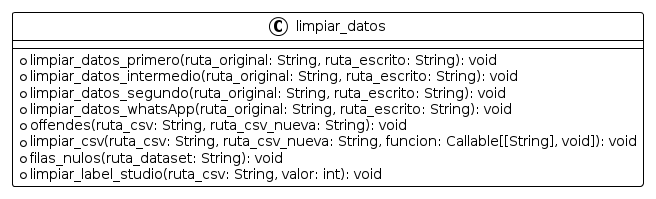
\includegraphics[width=0.65\textwidth]{capitulo5/figuras/fig1.png}
	\caption{Diagrama de clase del archivo limpiar\_datos
		\\\textit{Fuente: Elaboracion Propia}}
	\label{fig:uml1}
\end{figure}

\end{itemize}

%\textbf{Formato y Encadenamiento de Información}

La carpeta gestionarchivos contiene los archivos manejo\_archivos.py y convertir\_formato.py cada uno es importante para el uso de las funciones del archivo limpiar\_datos.py a continuacion se describen estos archivos:

\begin{itemize}

\item manejo\_archivos.py: Este archivo se encarga de la creación, copia, recorrido y vaciado de archivos en diferentes formatos. Para más detalles, consulte la figura \ref{fig:uml3}.

\begin{figure}[h!]
	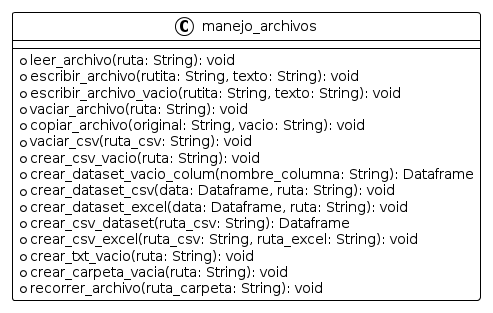
\includegraphics[width=0.65\textwidth]{capitulo5/figuras/fig3.png}
	\caption{Diagrama de clase del archivo manejo\_archivos
		\\\textit{Fuente: Elaboracion Propia}}
	\label{fig:uml3}
\end{figure}


\item convertir\_formato.py: Este archivo se ocupa de agrupar información de múltiples archivos para hacer uso de forma masiva de las funciones de limpieza definidas en el archivo limpiar\_datos.py, además de manejar el formato de los mismos cuando sea necesario. Para más detalles, consulte la figura \ref{fig:uml4}.

\begin{figure}[h!]
	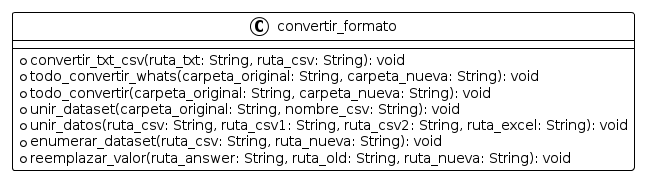
\includegraphics[width=0.8\textwidth]{capitulo5/figuras/fig4.png}
	\caption{Diagrama de clase del archivo convertir\_formato
		\\\textit{Fuente: Elaboracion Propia}}
	\label{fig:uml4}
\end{figure}

\end{itemize}

Es importante recordar que el preprocesamiento de datos varía según la fuente de los datos. Para más detalles sobre el proceso de limpieza de los datos provenientes de Facebook, consulte la figura \ref{fig:um12} (diagrama de actividades de Facebook) y el proceso de limpieza de datos provenientes de WhatsApp se puede apreciar en la figura \ref{fig:um13}(diagrama de actividades de Whatsapp).

\begin{figure}[h!]
	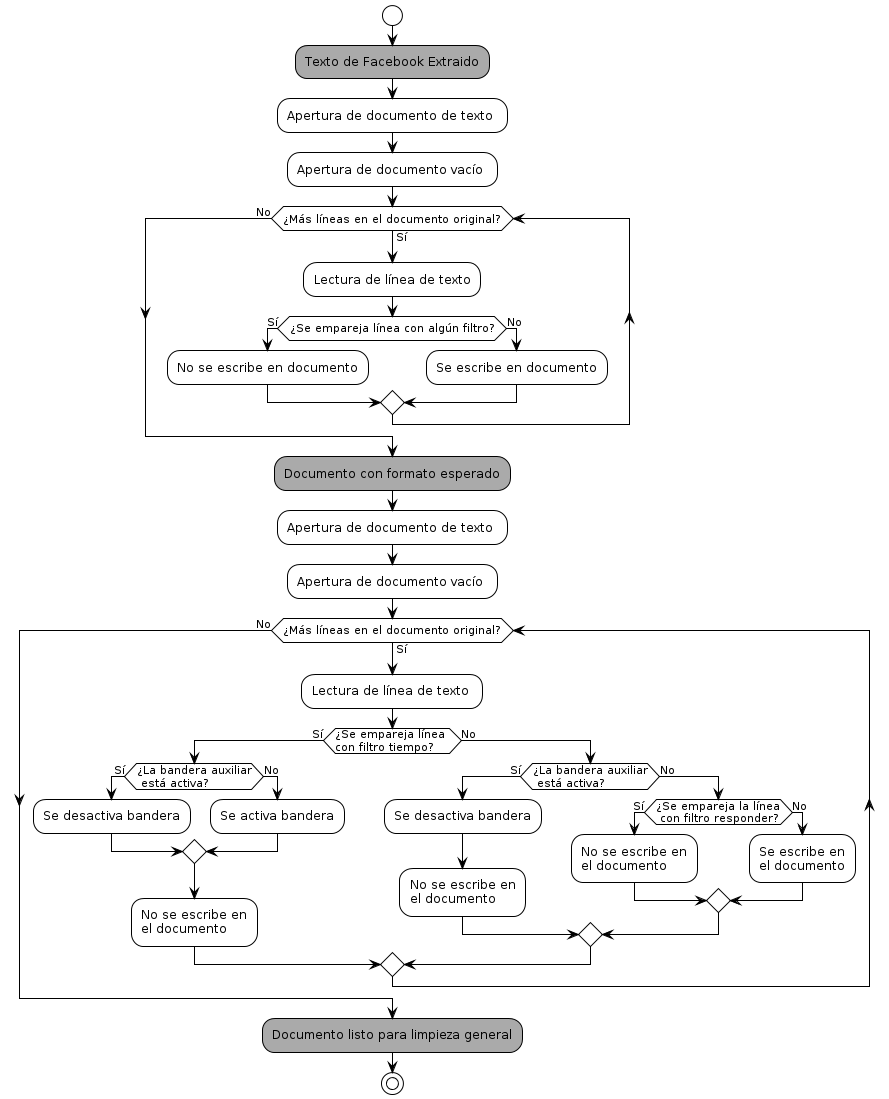
\includegraphics[width=1\textwidth]{capitulo5/figuras/prueba.png}
	\caption{Diagrama de actividades limpieza datos facebook
		\\\textit{Fuente: Elaboracion Propia}}
	\label{fig:um12}
\end{figure}

\begin{figure}[h!]
	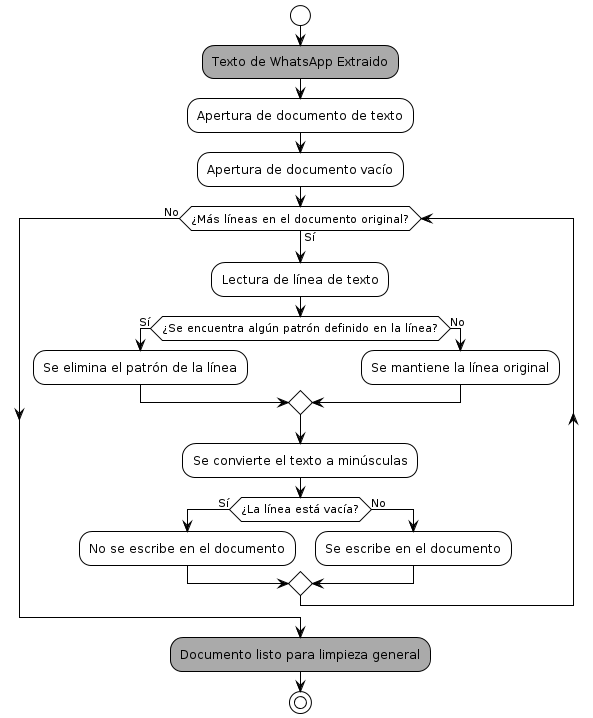
\includegraphics[width=0.7\textwidth]{capitulo5/figuras/part3.png}
	\caption{Diagrama de actividades limpieza datos whatsapp
		\\\textit{Fuente: Elaboracion Propia}}
	\label{fig:um13}
\end{figure}




\subsection{Implementación}
A continuación, se presenta el código fuente de los archivos detallados anteriormente en esta sección:

%\textbf{Limpieza de Datos}

%El archivo de la carpeta limpiezadataset se detalla a continuación:

El código fuente \ref{lst:c1} corresponde al archivo limpiar\_datos.py, donde se puede observar la implementación de la limpieza de datos extraídos de las redes sociales, se usaron expresiones regulares en la implementación de cada función. 

\lstinputlisting[language=Python,firstline=7,caption=Codigo fuente del archivo limpiar\_datos.py,label={lst:c1}]{capitulo5/codigo/limpiar_datos.py}

\vspace{-1.3em} % Ajusta el valor según sea necesario

\begin{figure}[h!]
	\centering % Incrementa el contador de lstlisting
	\textit{Fuente: Elaboración propia}
\end{figure}






La carpeta gestionarchivos almacena dos archivos y se enfoca en el tratamiento de archivos y formatos. En el código fuente \ref{lst:c3} se puede observar la implementación del archivo manejo\_archivos.py, que se encarga de crear, modificar, eliminar, y gestionar archivos en distintos formatos.

\lstinputlisting[language=Python,firstline=7,caption=Codigo fuente del archivo manejo\_archivos.py,label={lst:c3}]{capitulo5/codigo/manejo_archivos.py}
\vspace{-1.3em} % Ajusta el valor según sea necesario

\begin{figure}[h!]
	\centering % Incrementa el contador de lstlisting
	\textit{Fuente: Elaboración propia}
\end{figure}

En el código fuente \ref{lst:c4} se puede observar la implementación del último archivo de esta sección, convertir\_formato.py. Este archivo se encarga de recorrer múltiples archivos para compactar la información y realizar su conversión posterior. Además, se lleva a cabo el registro de cada archivo utilizado y de cada proceso realizado con este.

\lstinputlisting[language=Python,firstline=8,caption=Codigo fuente del archivo convertir\_formato.py,label={lst:c4}]{capitulo5/codigo/convertir_formato.py}
\vspace{-1.3em} % Ajusta el valor según sea necesario

\begin{figure}[h!]
	\centering % Incrementa el contador de lstlisting
	\textit{Fuente: Elaboración propia}
\end{figure}

\section{PREPROCESAMIENTO DE TEXTO}
En esta sección se detalla la implementación de cada paso realizado para el preprocesamiento de los datos, el cual se lleva a cabo después de la fase de limpieza de texto. En esta etapa, se trabaja con documentos de texto ya despojados de su formato original, facilitando su segmentación y tratamiento posterior. El objetivo principal del preprocesamiento es manejar la estructura interna del texto, segmentándolo en frases, oraciones o palabras, según sea más conveniente. El resultado de este proceso es un conjunto de datos limpio, útil y en uno de los formatos estándar aceptables para el uso del modelo de etiquetado. A continuación, se describe el archivo encargado del preprocesamiento de comentarios:

\begin{itemize}

\item corrector\_lenguaje.py: Este archivo aborda los aspectos generales de limpieza, que se pueden aplicar a varios tipos de información, independientemente de su fuente. Los detalles de este archivo se muestran en la figura \ref{fig:uml2}.

\begin{figure}[h!]
	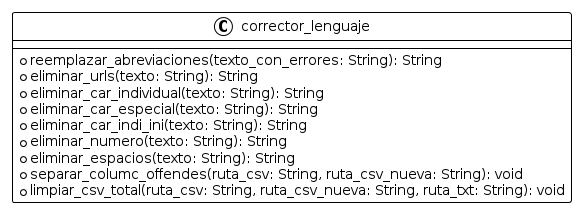
\includegraphics[width=0.65\textwidth]{capitulo5/figuras/fig2.png}
	\caption{Diagrama de clase del archivo corrector\_lenguaje
		\\\textit{Fuente: Elaboracion Propia}}
	\label{fig:uml2}
\end{figure}

\end{itemize}

La carpeta gestionarchivos contiene el archivo limpiar\_datos.py, que es utilizado en el archivo convertir\_formato.py. De manera similar, corrector\_lenguaje.py emplea el archivo manejo\_archivos.py, también ubicado en la misma carpeta. Esta organización permite que ambos archivos compartan la carpeta para aprovechar las funciones de tratamiento de formatos y la manipulación masiva de datos en múltiples archivos.
Una vez que los datos han pasado por los procesos de limpieza y preprocesamiento, se obtiene un producto final listo para ser utilizado en modelos de aprendizaje.



\subsection{Implementación}
A continuación, se presenta el código fuente del  archivo detallado anteriormente en esta sección:

El código fuente \ref{lst:c2} corresponde al archivo corrector\_lenguaje.py, que se encarga de la limpieza general de un conjunto de datos. Esto incluye la eliminación de URLs, caracteres especiales, números, entre otros elementos, utilizando la biblioteca re de Python.

\lstinputlisting[language=Python,firstline=7,caption=Codigo fuente del archivo corrector\_lenguaje.py,label={lst:c2}]{capitulo5/codigo/corrector_lenguaje.py}






\section{ETIQUETADO DE DATOS}
En este módulo se incluyen todos los pasos necesarios para el etiquetado de los datos adquiridos con el modelo BERT, su revisión y reetiquetado. El mismo contiene las siguientes secciones:

Etiquetado de Comentarios

La carpeta etiquetadodatos almacena los siguientes archivos:

\begin{itemize}

\item operacion\_dataset.py: Este archivo se encarga de diversas operaciones necesarias para el entrenamiento del modelo BERT, como la mezcla de datos, el conteo de clases y la división de conjuntos de datos. Para más detalles, consulte la figura 5.

------------------------------------------

figura 5

-----------------------------------------

\item bert\_multi.py: Este archivo se ocupa de la creación, configuración, entrenamiento y predicción, entre otras tareas específicas del modelo BERT. Para más detalles, consulte la figura 6.

---------------------------------------

figura 6

--------------------------------------

\end{itemize}

Reetiquetado y Revisión de Etiquetas

Para el reetiquetado de los conjuntos de datos, se utilizó la herramienta Label Studio, que acepta archivos en varios formatos como CSV y TSV. Esta herramienta proporciona una interfaz cómoda que agiliza el proceso de revisión, etiquetado y reetiquetado. Además, ofrece filtros y otras funciones que permiten realizar cambios en cualquier conjunto de datos, los cuales pueden exportarse en distintos formatos.



\subsection{Bert y el etiquetado de comentarios}
Durante la revisión del conjunto de datos ``Offendes'', se identificó que existian varias muestras que requerían reetiquetado, especialmente aquellas marcadas con lenguaje grosero. Por lo tanto, se revisó nuevamente todo el conjunto de datos, centrándose especialmente en las muestras con lenguaje grosero, y se procedió a reetiquetar manualmente teniendo en cuenta su utilidad y la percepción sobre si estos comentarios pertenecian a la categoria de groseros, ofensivos o no ofensivos en la sociedad boliviana.

De un total de 30,416 comentarios, 2,310 pertenecían a la clase de comentarios groseros pero no ofensivos. Se reetiquetaron 142 comentarios de esta clase y posteriormente se llevó a cabo la limpieza de este conjunto de datos para su uso adecuado.

El etiquetado de los conjuntos de datos de Facebook y WhatsApp se realizó después de la limpieza de los mismos. Para esta tarea, se utilizó la técnica de aprendizaje por transferencia, que consiste en aprovechar los conocimientos adquiridos en una tarea para mejorar el rendimiento en otra tarea relacionada pero diferente. En este caso, se empleó el dataset ``Offendes'' para afinar una versión reducida del modelo BERT, el cual fue inicialmente entrenado con grandes cantidades de texto no etiquetado, como páginas web, libros y artículos de noticias. A través de este proceso de entrenamiento masivo, el modelo aprende a comprender la estructura y el significado del lenguaje natural de manera general. Por lo tanto, cuando se adapta o afina para tareas específicas, como la clasificación de comentarios ofensivos, el modelo ya posee un conocimiento previo considerable del lenguaje, lo que permite mejorar su rendimiento en la tarea objetivo. Esto permitió que una muestra de aproximadamente 30,000 comentarios previamente etiquetados fuera utilizada para etiquetar los más de 78,000 comentarios recopilados de las redes sociales.

\begin{itemize}
 \item{Resultados del etiquetado con Bert}

Inicialmente, se utilizó el conjunto de datos ``Offendes'' para entrenar y afinar  el modelo BERT seleccionado, con el fin de etiquetar posteriormente el conjunto de datos recolectado de la región de los valles, centrándose específicamente en el departamento de Cochabamba. Los resultados del entrenamiento de BERT con ``Offendes'' se pueden apreciar en la Tabla \ref{tbl:bert}, donde en cantidad de muestras se detalla la cantidad de comentarios usados para el conjunto de entrenamiento, validación y prueba, en precisión la exactitud del modelo en su respectivo conjunto y en error las etiquetas que se marcaron incorrectamente en cada conjunto.

\begin{table}[!ht]
	\centering
	\begin{tabular}{|c|c|c|c|}
		\hline
		\textbf{Conjunto} & \textbf{Cantidad de muestras} & \textbf{Precisión} & \textbf{Error} \\ \hline
		Entrenamiento & 21169 & 0.9297 & 0.1969 \\ 
		Validación & 4536 & 0.8715 & 0.4100 \\ 
		Prueba & 4536 & 0.8748 & 0.3932 \\ \hline
		\textbf{Total} & 30241 & - & - \\ \hline
	\end{tabular}
	\caption{Resultados del entrenamiento de Bert con Offendes
		\\\textit{Fuente: Elaboración Propia}}
	\label{tbl:bert}
\end{table}


Bajo el resultado obtenido descrito en la Tabla \ref{tbl:bert}, se etiquetó el conjunto de datos de Cochabamba, cuyos resultados se detallan en la Tabla \ref{tbl:cochabamba}, donde la precisión es el resultado de la revisión manual realizada después del etiquetado. Finalmente despues de todo este proceso se etiquetaron los tres últimos conjuntos de datos restantes. En la tabla \ref{tbl:santacruz} se pueden observar los resultados del etiquetado del conjunto de datos de Santa Cruz, en la tabla \ref{tbl:lapaz} se presentan los resultados obtenidos para el conjunto de datos de La Paz, y finalmente, en la tabla \ref{tbl:whatsapp} se muestran los resultados obtenidos para el conjunto de datos de WhatsApp.


\begin{table}[!ht]
	\centering
	\begin{tabular}{|c|c|c|c|}
		\hline
		\textbf{Categorías} & \textbf{Cantidad} & \textbf{No de etiquetas cambiadas} & \textbf{Precisión (\%)} \\ \hline
		Ofensivos & 8199 & 3426 & 58.22 \\ 
		No ofensivos & 26856 & 1509 & 94.38 \\ 
		Groseros & 808 & 355 & 56.06 \\ \hline
		\textbf{Total} & 35863 & 5290 & \textbf{85.25} \\ \hline
	\end{tabular}
	\caption{Resultados del etiquetado de Bert para Cochabamba
		\\\textit{Fuente: Elaboración Propia}}
	\label{tbl:cochabamba}
\end{table}

\begin{table}[!ht]
	\centering
	\begin{tabular}{|c|c|c|}
		\hline
		\textbf{Categoría} & \textbf{Cantidad} & \textbf{Porcentaje (\%)} \\ \hline
		Ofensivo & 3171 & 22.33 \\ 
		No ofensivo & 10650 & 75.00 \\ 
		Grosero & 379 & 2.67 \\ \hline
		\textbf{Total} & 14200 & \textbf{100.00} \\ \hline
	\end{tabular}
	\caption{Resultados del etiquetado de Bert para Santa Cruz
		\\\textit{Fuente: Elaboración Propia}}
	\label{tbl:santacruz}
\end{table}


\begin{table}[!ht]
	\centering
	\begin{tabular}{|c|c|c|}
		\hline
		\textbf{Categoría} & \textbf{Cantidad} & \textbf{Porcentaje (\%)} \\ \hline
		Ofensivo & 4133 & 29.62 \\ 
		No ofensivo & 9379 & 67.18 \\ 
		Grosero & 449 & 3.21 \\ \hline
		\textbf{Total} & 13961 & \textbf{100.00} \\ \hline
	\end{tabular}
	\caption{Resultados del etiquetado de Bert para La Paz
		\\\textit{Fuente: Elaboración Propia}}
	\label{tbl:lapaz}
\end{table}

\begin{table}[!ht]
	\centering
	\begin{tabular}{|c|c|c|}
		\hline
		\textbf{Categoría} & \textbf{Cantidad} & \textbf{Porcentaje (\%)} \\ \hline
		Ofensivo & 2050 & 14.79 \\ 
		No ofensivo & 11129 & 80.31 \\ 
		Grosero & 680 & 4.90 \\ \hline
		\textbf{Total} & 13859 & \textbf{100.00} \\ \hline
	\end{tabular}
	\caption{Resultados del etiquetado de Bert para WhatsApp
		\\\textit{Fuente: Elaboración Propia}}
	\label{tbl:whatsapp}
\end{table}
\end{itemize}

\subsection{Implementación}
A continuación, se presenta el código fuente de cada archivo de la sección detallada:

%\textbf{Etiquetado de comentarios}

En la carpeta etiquetadodatos se almacenan dos archivos, el código fuente \ref{lst:c5} corresponde al archivo bert\_multi.py, donde se puede observar la implementación del modelo Bert y cualquier función necesaria para el guardado de datos y del modelo mismo.

\lstinputlisting[language=Python,firstline=11,caption=Codigo fuente del archivo bert\_multi.py,label={lst:c5}]{capitulo5/codigo/bert_multi.py}
\vspace{-1.3em} % Ajusta el valor según sea necesario

\begin{figure}[h!]
	\centering % Incrementa el contador de lstlisting
	\textit{Fuente: Elaboración propia}
\end{figure}

El código fuente \ref{lst:c6} corresponde al archivo operacion\_dataset.py, que contiene las funciones implementadas para las operaciones necesarias en los conjuntos de datos utilizados por el modelo BERT.


\lstinputlisting[language=Python,firstline=7,caption=Codigo fuente del archivo operacion\_dataset.py,label={lst:c6}]{capitulo5/codigo/operacion_dataset.py}
\vspace{-1.3em} % Ajusta el valor según sea necesario

\begin{figure}[h!]
	\centering % Incrementa el contador de lstlisting
	\textit{Fuente: Elaboración propia}
\end{figure}
\section{INGENIERÍA DE CARACTERÍSTICAS}
En esta sección se detallan los pasos para la división del conjunto de datos, cuyos elementos textuales serán posteriormente transformados en representaciones numéricas.

\subsection{División de comentarios}
Se trabajó con una porción del conjunto de datos total, específicamente con 35,000 muestras, las cuales se dividieron en tres partes: el conjunto de entrenamiento, el conjunto de prueba y el conjunto de validación. Las proporciones correspondientes a cada porción se pueden visualizar en la tabla \ref{tbl:conjuntos}, para asegurar la uniformidad en la distribución de clases, lo cual es crucial para el rendimiento del modelo, se creó este conjunto de datos priorizando una cantidad de muestras equilibrada para cada clase.


\begin{table}[!ht]
	\centering
	\begin{tabular}{|c|c|c|c|c|}
		\hline
		\textbf{Conjunto} & \textbf{Ofensivo} & \textbf{No ofensivo} & \textbf{Grosero} & \textbf{Porcentaje (\%)} \\ \hline
		Entrenamiento & 10250 & 10250 & 4000 & 24500 = 70\% \\ 
		Validación & 2125 & 2125 & 1000 & 5250 = 15\% \\ 
		Prueba & 2580 & 2572 & 98 & 5250 = 15\% \\ \hline
		\textbf{Total} & 14955 & 14947 & 5098 & \textbf{35.000 = 100\%} \\ \hline
	\end{tabular}
	\caption{División del conjunto de datos
		\\\textit{Fuente: Elaboración Propia}}
	\label{tbl:conjuntos}
\end{table}


Como se puede observar en la tabla \ref{tbl:conjuntos} la cantidad de clases en los conjuntos de datos no es uniforme para la categoría de lenguaje grosero, esto debido a que la cantidad de muestras totales para esta categoría no sobrepasa los 6000 ejemplares y por esa razón se priorizo otorgarle la mayor cantidad de muestras posibles a los conjuntos de entrenamiento y validación.
\subsection{Archivos de la representación textual}
A continuación, se detallan los diagramas de clases desarrollados para esta fase.

 La carpeta entrenarmodelos contiene cinco archivos, de los cuales dos son responsables de la división del conjunto de datos y su transformación en vectores numéricos densos, también conocidos como embeddings. Los archivos correspondientes son los siguientes: 

\begin{itemize}

\item creando\_dataset.py: Se encarga de la división de los conjuntos de datos en subconjuntos para el entrenamiento, la validación y la prueba, asegurando que cada una de las tres clases esté representada de la mejor manera para el entrenamiento de los modelos. También permite la visualización del estado del conjunto de datos, como el tamaño de secuencias y la bolsa de palabras, para mas detalles ver la figura \ref{fig:uml7}.

\begin{figure}
	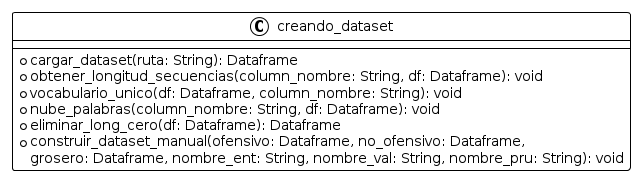
\includegraphics[width=0.65\textwidth]{capitulo5/figuras/fig7.png}
	\caption{Diagrama de clase del archivo creando\_dataset
		\\\textit{Fuente: Elaboración Propia}}
	\label{fig:uml7}
\end{figure}

\item preparar\_datos.py: Recibe el conjunto de datos en formato .CSV mismo que contiene comentarios textuales y sus etiquetas correspondientes. Convierte estos datos a listas para realizar procesos de tokenización, padding, carga de embeddings y procesamiento de embeddings, después de establecer los hiperparametros necesarios como el tamaño máximo de secuencia, el número máximo de palabras y la dimensión de los embeddings, además se crean métodos para el armado de la capa de embedding, compilación, entrenamiento, evaluación y graficación de los modelos, para mas detalles ver la figura \ref{fig:uml8}.

\begin{figure}[h!]
	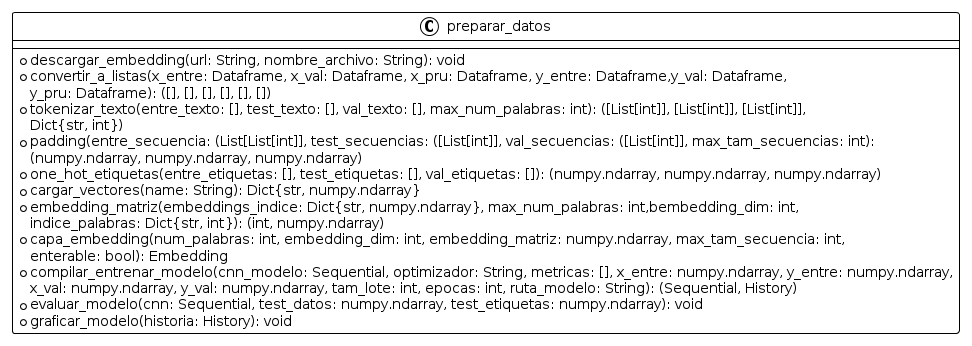
\includegraphics[width=0.95\textwidth]{capitulo5/figuras/fig8.png}
	\caption{Diagrama de clase del archivo preparar\_datos
		\\\textit{Fuente: Elaboración Propia}}
	\label{fig:uml8}
\end{figure}

\end{itemize}

Estos archivos abarcan los procesos de distribución equilibrada de clases, visualización de secuencias, conteo de palabras y creación de la bolsa de palabras del conjunto de datos final, además del manejo de los embeddings. Para la carga de embeddings, se utilizó la versión paga de Colab, debido a la necesidad de usar una mayor capacidad de memoria RAM.

\subsection{Implementación}
A continuación, se presenta el código fuente de los  archivos detallados anteriormente:

En el código fuente \ref{lst:c7} se puede observar la implementación del primer archivo, creando\_dataset.py, que visualiza el estado del conjunto de datos y lo divide manualmente, priorizando una distribución equilibrada entre las clases.

\lstinputlisting[language=Python,firstline=8,caption=Codigo fuente del archivo creando\_dataset.py,label={lst:c7}]{capitulo5/codigo/creando_dataset.py}

En el código fuente \ref{lst:c8} se observa la implementación del archivo preparar\_datos.py, que prepara la entrada final lista para la primera capa de los modelos propuestos. Esto implica la representación del texto en formas numéricas, en este caso, mediante embeddings. Además contiene funciones de armado, compilación, entrenamiento, entre otras funciones para los modelos de redes convolucionales

\lstinputlisting[language=Python,firstline=9,caption=Codigo fuente del archivo preparar\_datos,label={lst:c8}]{capitulo5/codigo/preparar_datos.py}

\section{MODELADO}
Se detallan los diferentes diagramas de clases de los restantes tres archivos de la carpeta entrenarmodelos, estos archivos contienen la implementación de los diversos modelos propuestos:

\begin{itemize}

\item cnn\_tres.py: Crea los modelos de redes convolucionales propuestos con una arquitectura base de tres capas, para más detalles ver la figura \ref{fig:uml9}.

\begin{figure}[h!]
	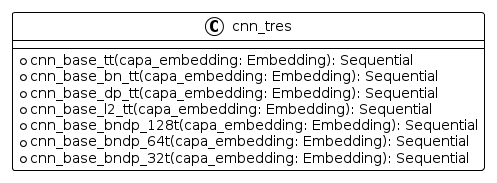
\includegraphics[width=0.65\textwidth]{capitulo5/figuras/fig9.png}
	\caption[Diagrama de clase del archivo cnn\_tres]{Diagrama de clase del archivo cnn\_tres
		\\\textit{Fuente: Elaboración Propia}}
	\label{fig:uml9}
\end{figure}

\item cnn\_four.py: Crea los modelos de redes convolucionales propuestos con una arquitectura base de cuatro capas, para más detalles ver la figura \ref{fig:uml10}.

\begin{figure}[h!]
	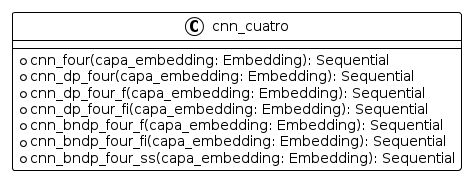
\includegraphics[width=0.6\textwidth]{capitulo5/figuras/fig10.png}
	\caption[Diagrama de clase del archivo cnn\_cuatro]{Diagrama de clase del archivo cnn\_cuatro
		\\\textit{Fuente: Elaboración Propia}}
	\label{fig:uml10}
\end{figure}

\item cnn\_dos.py: Crea los modelos de redes convolucionales propuestos con una arquitectura base de dos capas, para más detalles ver la figura \ref{fig:uml11}.

\begin{figure}[h!]
	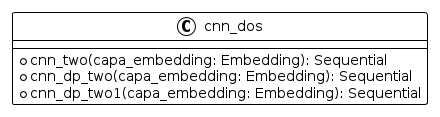
\includegraphics[width=0.5\textwidth]{capitulo5/figuras/fig11.png}
	\caption[Diagrama de clase del archivo cnn\_dos]{Diagrama de clase del archivo cnn\_dos
		\\\textit{Fuente: Elaboración Propia}}
	\label{fig:uml11}
\end{figure}

\end{itemize}

Para cada modelo propuesto, se guarda una copia en cualquier época durante el entrenamiento en la que la pérdida del conjunto de validación disminuya. Además, para mayor comodidad, se almacena todo el historial de entrenamiento de cada modelo, permitiendo visualizar su avance y realizar comparaciones con otros modelos.


\subsection{Implementación}
A continuación se detalla la implementación de cada archivo detallado en esta seccion:

En el código fuente \ref{lst:c9} se observa la implementación de todos los modelos de redes neuronales convolucionales basados en el modelo base propuesto, contenido en el archivo cnn\_tres.py.

\lstinputlisting[language=Python,firstline=7,caption=Codigo fuente del archivo cnn\_tres.py,label={lst:c9}]{capitulo5/codigo/cnn_tres.py}

En el código fuente \ref{lst:c10} se observa la implementación de los modelos propuestos con una capa convolucional mayor a la arquitectura base. Todo esto se encuentra en el archivo cnn\_cuatro.py

\lstinputlisting[language=Python,firstline=7,caption=Codigo fuente del archivo cnn\_cuatro.py,label={lst:c10}]{capitulo5/codigo/cnn_cuatro.py}

Finalmente, en el código fuente \ref{lst:c11} se observa la implementación de todos los modelos de redes neuronales convolucionales con dos capas, contenido en el archivo cnn\_dos.py.

\lstinputlisting[language=Python,firstline=7,caption=Codigo fuente del archivo cnn\_dos.py,label={lst:c11}]{capitulo5/codigo/cnn_dos.py}



\subsection{Desarrollo de los modelos convolucionales}
Para establecer la arquitectura base, los hiperparámetros y cualquier configuración necesaria en los modelos base, se aprovechó principalmente la teoría detallada en este proyecto, así como la documentación expuesta de las herramientas en uso, donde se pueden observar los valores que pueden establecerse. Además, se tuvieron en cuenta trabajos relacionados o similares a la tarea en cuestión. Se optó por utilizar una red neuronal convolucional 1D debido a la naturaleza de los datos textuales. Los hiperparámetros específicos se detallarán más adelante.

\begin{itemize}
	\item Hiperparametros de los modelos
\end{itemize}
Los hiperparámetros utilizados se pueden dividir en dos categorías. En la primera se encuentran los hiperparámetros constantes, que no se modificaron durante ni después de las pruebas, esta sección se enfocara en estos hiperparámetros. Respecto a la segunda categoria donde se trata a los hiperparámetros que se modificaron durante las pruebas se detallarán al momento de describir los modelos y sus resultados.

En la tabla \ref{tbl:3} se pueden observar los hiperparámetros utilizados para la capa de embedding en cada uno de los modelos convolucionales propuestos.

\begin{table}[!ht]
	\centering
	\begin{tabular}{|c|c|}
		\hline
		\textbf{Hiperparametro} & \textbf{Valor} \\ \hline
		max\_tam\_secuencia & 150 \\ \hline
		max\_num\_palabras  & 40000 \\ \hline
		embedding\_dim  & 300 \\ \hline
		max\_num\_palabras & 40000 \\ \hline
		embedding\_matriz & 30270 x 300 \\ \hline
		entrenable & False \\ \hline
	\end{tabular}
	\caption{Detalle Hiperparametros y valores usados para la capa de embedding
		\\\textit{Fuente: Elaboracion Propia}}
	\label{tbl:3}
\end{table}

Para las capas restantes, como las capas de convolución, se detallan los hiperparámetros constantes en la tabla \ref{tbl:4}.

\begin{table}[!ht]
	\centering
	\begin{tabular}{|c|c|}
		\hline
		\textbf{Hiperparametro } & \textbf{Valor} \\ \hline
		Optimizador & 'rmsprop' \\ \hline
		Batch\_size & 128 \\ \hline
		Epoca & 150 \\ \hline
		funcion\_activacion en capas convolucionales & 'relu' \\ \hline
		funcion\_activacion en capa densa intermedia & 'relu' \\ \hline
		funcion\_activacion en capa densa de salida & 'softmax' \\ \hline
	\end{tabular}
	\caption{Detalle Hiperparametros y valores usados para las capas restantes
		\\\textit{Fuente: Elaboracion Propia}}
	\label{tbl:4}
\end{table}

\begin{itemize}
	\item Primera iteración
\end{itemize}

En la primera iteración de las pruebas, se utilizó una red convolucional 1D con tres capas de convolución, dos capas de maxpooling, una capa de globalmaxpooling y dos capas densas. Esta arquitectura se puede observar con más detalle en la la tabla \ref{tbl:5}, la misma constituye la arquitectura base del modelo cnn\_base\_tt.


\begin{table}[!ht]
	\centering
	\begin{tabular}{|c|c|c|}
		\hline
		\textbf{Tipo de capa } & \textbf{Hiperparámetro } & \textbf{Valor} \\ \hline
		1ra capa convolucional 1D & num\_filtros, tam\_filtros, stride & 32, 3, 1 \\ \hline
		1ra capa maxpooling & tam\_pool, pool\_stride & 2, 2 \\ \hline
		2da capa convolucional 1D & num\_filtros, tam\_filtros, stride & 64, 5, 1 \\ \hline
		2da capa maxpooling & tam\_pool, pool\_stride & 2, 2 \\ \hline
		3ra capa convolucional 1D & num\_filtros, tam\_filtros, stride & 128, 5, 1 \\ \hline
		1ra capa densa intermedia & num\_neuronas & 128 \\ \hline
		2da capa densa de salida & num\_neuronas & 3 \\ \hline
	\end{tabular}
	\caption{Detalle arquitectura del modelo base
		\\\textit{Fuente: Elaboracion Propia}}
	\label{tbl:5}
\end{table}

De igual forma se detallan los modelos base utilizados junto con las técnicas de regularización aplicadas a cada uno. Se eligieron tres tipos de técnicas de regularización: normalización por lotes (batch normalization), regularización L2 y dropout. En esta iteración, se aplicó un tipo de regularización a cada capa convolucional. Los detalles  sobre cada uno de los modelos regularizados se presentan a continuación:

\begin{itemize}
	
	\item Modelo cnn\_base\_bn\_tt: Se aplicó normalización por lotes (batch normalization) a cada capa convolucional y a la capa densa intermedia, para más detalles ver la tabla \ref{tbl:cnn_base_bn_tt}.
	
	\begin{table}[!ht]
		\centering
		\begin{tabular}{|c|c|c|}
			\hline
			\textbf{Tipo de capa} & \textbf{Hiperparámetro} & \textbf{Valor} \\ \hline
			1ra capa convolucional 1D & num\_filtros, tam\_filtros, stride & 32, 3, 1 \\ \hline
			1ra capa BatchNormalization & - & - \\ \hline
			1ra capa maxpooling & tam\_pool, pool\_stride & 2, 2 \\ \hline
			2da capa convolucional 1D & num\_filtros, tam\_filtros, stride & 64, 5, 1 \\ \hline
			2da capa BatchNormalization & - & - \\ \hline
			2da capa maxpooling & tam\_pool, pool\_stride & 2, 2 \\ \hline
			3ra capa convolucional 1D & num\_filtros, tam\_filtros, stride & 128, 5, 1 \\ \hline
			3ra capa BatchNormalization & - & - \\ \hline
			1ra capa densa intermedia & num\_neuronas & 128 \\ \hline
			4ta capa BatchNormalization & - & - \\ \hline
			2da capa densa de salida & num\_neuronas & 3 \\ \hline
		\end{tabular}
		\caption{Arquitectura del modelo cnn\_base\_bn\_tt
			\\\textit{Fuente: Elaboracion Propia}}
		\label{tbl:cnn_base_bn_tt}
	\end{table}
	
	
	\item  Modelo cnn\_base\_dp\_tt: Se aplicó un dropout al 30\% a todas las capas convolucionales y un dropout al 50\% a la capa densa intermedia, para más detalles ver la tabla \ref{tbl:cnn_base_dp_tt}.
	
	\begin{table}[!ht]
		\centering
		\begin{tabular}{|c|c|c|}
			\hline
			\textbf{Tipo de capa} & \textbf{Hiperparámetro} & \textbf{Valor} \\ \hline
			1ra capa convolucional 1D & num\_filtros, tam\_filtros, stride & 32, 3, 1 \\ \hline
			1ra capa Dropout & tasa & 0.3 \\ \hline
			1ra capa maxpooling & tam\_pool, pool\_stride & 2, 2 \\ \hline
			2da capa convolucional 1D & num\_filtros, tam\_filtros, stride & 64, 5, 1 \\ \hline
			2da capa Dropout & tasa & 0.3 \\ \hline
			2da capa maxpooling & tam\_pool, pool\_stride & 2, 2 \\ \hline
			3ra capa convolucional 1D & num\_filtros, tam\_filtros, stride & 128, 5, 1 \\ \hline
			3ra capa Dropout & tasa & 0.3 \\ \hline
			1ra capa densa intermedia & num\_neuronas & 128 \\ \hline
			4ta capa Dropout & tasa & 0.5 \\ \hline
			2da capa densa de salida & num\_neuronas & 3 \\ \hline
		\end{tabular}
		\caption{Arquitectura del modelo cnn\_base\_dp\_tt
			\\\textit{Fuente: Elaboracion Propia}}
		\label{tbl:cnn_base_dp_tt}
	\end{table}
	
	
	\item  Modelo cnn\_base\_l2\_tt: Se aplicó regularización L2 con un valor de 0,05 a cada capa convolucional y a la capa densa intermedia, para más detalles ver la tabla \ref{tbl:cnn_base_l2_tt}.
	
	\begin{table}[!ht]
		\centering
		\begin{tabular}{|c|c|c|}
			\hline
			\textbf{Tipo de capa} & \textbf{Hiperparámetro} & \textbf{Valor} \\ \hline
			1ra capa convolucional 1D & num\_filtros, tam\_filtros, stride, L2 & 32, 3, 1, 0.05 \\ \hline
			1ra capa maxpooling & tam\_pool, pool\_stride & 2, 2 \\ \hline
			2da capa convolucional 1D & num\_filtros, tam\_filtros, stride, L2 & 64, 5, 1, 0.05 \\ \hline
			2da capa maxpooling & tam\_pool, pool\_stride & 2, 2 \\ \hline
			3ra capa convolucional 1D & num\_filtros, tam\_filtros, stride, L2 & 128, 5, 1, 0.05 \\ \hline
			1ra capa densa intermedia & num\_neuronas, L2 & 128, 0.05 \\ \hline
			2da capa densa de salida & num\_neuronas & 3 \\ \hline
		\end{tabular}
		\caption{Arquitectura del modelo cnn\_base\_l2\_tt
			\\\textit{Fuente: Elaboracion Propia}}
		\label{tbl:cnn_base_l2_tt}
	\end{table}
	
	
\end{itemize}

También se utilizaron modelos base con dos técnicas de regularización simultáneamente. Se mantuvieron las mismas características en cuanto a la arquitectura, pero se modificó la capa densa intermedia a 64 y 32 neuronas. A continuación, se detallan estos modelos:

\begin{itemize}
	
	\item Modelo cnn\_base\_bndp\_128tt: Se aplicó normalización por lotes (batch normalization) y dropout a cada capa convolucional y a la capa densa intermedia, para más detalles ver la tabla \ref{tbl:cnn_base_bndp_128tt}.
	
	\begin{table}[!ht]
		\centering
		\begin{tabular}{|c|c|c|}
			\hline
			\textbf{Tipo de capa} & \textbf{Hiperparámetro} & \textbf{Valor} \\ \hline
			1ra capa convolucional 1D & num\_filtros, tam\_filtros, stride & 32, 3, 1 \\ \hline
			1ra capa BatchNormalization & - & - \\ \hline
			1ra capa Dropout & tasa & 0.3 \\ \hline
			1ra capa maxpooling & tam\_pool, pool\_stride & 2, 2 \\ \hline
			2da capa convolucional 1D & num\_filtros, tam\_filtros, stride & 64, 5, 1 \\ \hline
			2da capa BatchNormalization & - & - \\ \hline
			2da capa Dropout & tasa & 0.3 \\ \hline
			2da capa maxpooling & tam\_pool, pool\_stride & 2, 2 \\ \hline
			3ra capa convolucional 1D & num\_filtros, tam\_filtros, stride & 128, 5, 1 \\ \hline
			3ra capa BatchNormalization & - & - \\ \hline
			3ra capa Dropout & tasa & 0.3 \\ \hline
			1ra capa densa intermedia & num\_neuronas & 128 \\ \hline
			4ta capa Dropout & tasa & 0.5 \\ \hline
			2da capa densa de salida & num\_neuronas & 3 \\ \hline
		\end{tabular}
		\caption{Arquitectura del modelo cnn\_base\_bndp\_128tt
			\\\textit{Fuente: Elaboracion Propia}}
		\label{tbl:cnn_base_bndp_128tt}
	\end{table}
	
	
	\item Modelo cnn\_base\_bndp\_64tt: Se aplicó normalización por lotes (batch normalization) y dropout a cada capa convolucional y dropout a la primera capa densa intermedia donde se redujo la cantidad de neuronas a 64, para más detalles ver la tabla \ref{tbl:cnn_base_bndp_64tt}.
	
	\begin{table}[!ht]
		\centering
		\begin{tabular}{|c|c|c|}
			\hline
			\textbf{Tipo de capa} & \textbf{Hiperparámetro} & \textbf{Valor} \\ \hline
			1ra capa convolucional 1D & num\_filtros, tam\_filtros, stride & 32, 3, 1 \\ \hline
			1ra capa BatchNormalization & - & - \\ \hline
			1ra capa Dropout & tasa & 0.3 \\ \hline
			1ra capa maxpooling & tam\_pool, pool\_stride & 2, 2 \\ \hline
			2da capa convolucional 1D & num\_filtros, tam\_filtros, stride & 64, 5, 1 \\ \hline
			2da capa BatchNormalization & - & - \\ \hline
			2da capa Dropout & tasa & 0.3 \\ \hline
			2da capa maxpooling & tam\_pool, pool\_stride & 2, 2 \\ \hline
			3ra capa convolucional 1D & num\_filtros, tam\_filtros, stride & 128, 5, 1 \\ \hline
			3ra capa BatchNormalization & - & - \\ \hline
			3ra capa Dropout & tasa & 0.3 \\ \hline
			1ra capa densa intermedia & num\_neuronas & 64 \\ \hline
			4ta capa Dropout & tasa & 0.5 \\ \hline
			2da capa densa de salida & num\_neuronas & 3 \\ \hline
		\end{tabular}
		\caption{Arquitectura del modelo cnn\_base\_bndp\_64tt
			\\\textit{Fuente: Elaboracion Propia}}
		\label{tbl:cnn_base_bndp_64tt}
	\end{table}
	
	
	\item Modelo cnn\_base\_bndp\_32tt: Se aplicó normalización por lotes (batch normalization) y dropout a cada capa convolucional y dropout a la primera capa densa intermedia, donde se redujo la cantidad de neuronas a 32, para más detalles ver la tabla \ref{tbl:cnn_base_bndp_32tt}.
	
	\begin{table}[!ht]
		\centering
		\begin{tabular}{|c|c|c|}
			\hline
			\textbf{Tipo de capa} & \textbf{Hiperparámetro} & \textbf{Valor} \\ \hline
			1ra capa convolucional 1D & num\_filtros, tam\_filtros, stride & 32, 3, 1 \\ \hline
			1ra capa BatchNormalization & - & - \\ \hline
			1ra capa Dropout & tasa & 0.3 \\ \hline
			1ra capa maxpooling & tam\_pool, pool\_stride & 2, 2 \\ \hline
			2da capa convolucional 1D & num\_filtros, tam\_filtros, stride & 64, 5, 1 \\ \hline
			2da capa BatchNormalization & - & - \\ \hline
			2da capa Dropout & tasa & 0.3 \\ \hline
			2da capa maxpooling & tam\_pool, pool\_stride & 2, 2 \\ \hline
			3ra capa convolucional 1D & num\_filtros, tam\_filtros, stride & 128, 5, 1 \\ \hline
			3ra capa BatchNormalization & - & - \\ \hline
			3ra capa Dropout & tasa & 0.3 \\ \hline
			1ra capa densa intermedia & num\_neuronas & 32 \\ \hline
			4ta capa Dropout & tasa & 0.5 \\ \hline
			2da capa densa de salida & num\_neuronas & 3 \\ \hline
		\end{tabular}
		\caption{Arquitectura del modelo cnn\_base\_bndp\_32tt
			\\\textit{Fuente: Elaboracion Propia}}
		\label{tbl:cnn_base_bndp_32tt}
	\end{table}
	
	
\end{itemize}

\begin{itemize}
	\item Segunda iteración
\end{itemize}

En esta iteración se realizaron cambios en la arquitectura de la red convolucional base, principalmente en la cantidad de capas de convolución y el pool\_stride. Los detalles de la arquitectura del modelo cnn\_four se encuentran en la tabla \ref{tbl:9}.

\begin{table}[!ht]
	\centering
	\begin{tabular}{|c|c|c|}
		\hline
		\textbf{Tipo de capa} & \textbf{Hiperparámetro} & \textbf{Valor} \\ \hline
		1ra capa convolucional 1D & num\_filtros, tam\_filtros, stride & 32, 3, 1 \\ \hline
		1ra capa maxpooling & tam\_pool, pool\_stride & 2, 1 \\ \hline
		2da capa convolucional 1D & num\_filtros, tam\_filtros, stride & 64, 5, 1 \\ \hline
		2da capa maxpooling & tam\_pool, pool\_stride & 2, 1 \\ \hline
		3ra capa convolucional 1D & num\_filtros, tam\_filtros, stride & 128, 5, 1 \\ \hline
		3ra capa maxpooling & tam\_pool, pool\_stride & 2, 1 \\ \hline
		4ra capa convolucional 1D & num\_filtros, tam\_filtros, stride & 256, 7, 1 \\ \hline
		1ra capa densa intermedia & num\_neuronas & 128 \\ \hline
		2da capa densa de salida & num\_neuronas & 3 \\ \hline
	\end{tabular}
	\caption{Detalle de la arquitectura de cuatro capas
	\\\textit{Fuente: Elaboracion Propia}}
	\label{tbl:9}
\end{table}

Todos los modelos propuestos a continuación comparten esta arquitectura base con métodos de regularización adicionales:

\begin{itemize}
	
	\item Modelo cnn\_dp\_four: Incluye dropout al 30\% después de cada capa convolucional y dropout al 50\% después de la capa densa intermedia, para más detalles ver tabla \ref{tbl:cnn_dp_four}.
	
	\begin{table}[!ht]
		\centering
		\begin{tabular}{|c|c|c|}
			\hline
			\textbf{Tipo de capa} & \textbf{Hiperparámetro} & \textbf{Valor} \\ \hline
			1ra capa convolucional 1D & num\_filtros, tam\_filtros, stride & 32, 3, 1 \\ \hline
			1ra capa Dropout & tasa & 0.3 \\ \hline
			1ra capa maxpooling & tam\_pool, pool\_stride & 2, 1 \\ \hline
			2da capa convolucional 1D & num\_filtros, tam\_filtros, stride & 64, 5, 1 \\ \hline
			2da capa Dropout & tasa & 0.3 \\ \hline
			2da capa maxpooling & tam\_pool, pool\_stride & 2, 1 \\ \hline
			3ra capa convolucional 1D & num\_filtros, tam\_filtros, stride & 128, 5, 1 \\ \hline
			3ra capa Dropout & tasa & 0.3 \\ \hline
			3ra capa maxpooling & tam\_pool, pool\_stride & 2, 1 \\ \hline
			4ta capa convolucional 1D & num\_filtros, tam\_filtros, stride & 256, 7, 1 \\ \hline
			4ta capa Dropout & tasa & 0.3 \\ \hline
			1ra capa densa intermedia & num\_neuronas & 128 \\ \hline
			5ta capa Dropout & tasa & 0.5 \\ \hline
			2da capa densa de salida & num\_neuronas & 3 \\ \hline
		\end{tabular}
		\caption{Arquitectura del modelo cnn\_dp\_four
			\\\textit{Fuente: Elaboracion Propia}}
		\label{tbl:cnn_dp_four}
	\end{table}
	
	
	\item Modelo cnn\_dp\_four\_f: Incluye dropout al 40\% después de cada capa convolucional y dropout al 50\% después de la capa densa intermedia, para más detalles ver la tabla \ref{tbl:cnn_dp_four_f}.
	
	\begin{table}[!ht]
		\centering
		\begin{tabular}{|c|c|c|}
			\hline
			\textbf{Tipo de capa} & \textbf{Hiperparámetro} & \textbf{Valor} \\ \hline
			1ra capa convolucional 1D & num\_filtros, tam\_filtros, stride & 32, 3, 1 \\ \hline
			1ra capa Dropout & tasa & 0.4 \\ \hline
			1ra capa maxpooling & tam\_pool, pool\_stride & 2, 1 \\ \hline
			2da capa convolucional 1D & num\_filtros, tam\_filtros, stride & 64, 5, 1 \\ \hline
			2da capa Dropout & tasa & 0.4 \\ \hline
			2da capa maxpooling & tam\_pool, pool\_stride & 2, 1 \\ \hline
			3ra capa convolucional 1D & num\_filtros, tam\_filtros, stride & 128, 5, 1 \\ \hline
			3ra capa Dropout & tasa & 0.4 \\ \hline
			3ra capa maxpooling & tam\_pool, pool\_stride & 2, 1 \\ \hline
			4ta capa convolucional 1D & num\_filtros, tam\_filtros, stride & 256, 7, 1 \\ \hline
			4ta capa Dropout & tasa & 0.4 \\ \hline
			1ra capa densa intermedia & num\_neuronas & 128 \\ \hline
			5ta capa Dropout & tasa & 0.5 \\ \hline
			2da capa densa de salida & num\_neuronas & 3 \\ \hline
		\end{tabular}
		\caption{Arquitectura del modelo cnn\_dp\_four\_f
			\\\textit{Fuente: Elaboracion Propia}}
		\label{tbl:cnn_dp_four_f}
	\end{table}
	
	
	\item Modelo cnn\_dp\_four\_fi: Incluye dropout al 50\% después de cada capa convolucional y después de la capa densa intermedia, para más detalles ver la tabla \ref{tbl:cnn_dp_four_fi}.
	
	\begin{table}[!ht]
		\centering
		\begin{tabular}{|c|c|c|}
			\hline
			\textbf{Tipo de capa} & \textbf{Hiperparámetro} & \textbf{Valor} \\ \hline
			1ra capa convolucional 1D & num\_filtros, tam\_filtros, stride & 32, 3, 1 \\ \hline
			1ra capa Dropout & tasa & 0.5 \\ \hline
			1ra capa maxpooling & tam\_pool, pool\_stride & 2, 1 \\ \hline
			2da capa convolucional 1D & num\_filtros, tam\_filtros, stride & 64, 5, 1 \\ \hline
			2da capa Dropout & tasa & 0.5 \\ \hline
			2da capa maxpooling & tam\_pool, pool\_stride & 2, 1 \\ \hline
			3ra capa convolucional 1D & num\_filtros, tam\_filtros, stride & 128, 5, 1 \\ \hline
			3ra capa Dropout & tasa & 0.5 \\ \hline
			3ra capa maxpooling & tam\_pool, pool\_stride & 2, 1 \\ \hline
			4ta capa convolucional 1D & num\_filtros, tam\_filtros, stride & 256, 7, 1 \\ \hline
			4ta capa Dropout & tasa & 0.5 \\ \hline
			1ra capa densa intermedia & num\_neuronas & 128 \\ \hline
			5ta capa Dropout & tasa & 0.5 \\ \hline
			2da capa densa de salida & num\_neuronas & 3 \\ \hline
		\end{tabular}
		\caption{Arquitectura del modelo cnn\_dp\_four\_fi
			\\\textit{Fuente: Elaboracion Propia}}
		\label{tbl:cnn_dp_four_fi}
	\end{table}
	
	
	\item Modelo cnn\_bndp\_four\_f: Incluye dropout al 40\% después de cada capa convolucional y dropout al 50\% después de la capa densa intermedia, más batch normalization en dos capas convolucionales, para más detalles ver la tabla \ref{tbl:cnn_bndp_four_f}.
	
	\begin{table}[!ht]
		\centering
		\begin{tabular}{|c|c|c|}
			\hline
			\textbf{Tipo de capa} & \textbf{Hiperparámetro} & \textbf{Valor} \\ \hline
			1ra capa convolucional 1D & num\_filtros, tam\_filtros, stride & 32, 3, 1 \\ \hline
			1ra capa BatchNormalization & - & - \\ \hline
			1ra capa Dropout & tasa & 0.5 \\ \hline
			1ra capa maxpooling & tam\_pool, pool\_stride & 2, 1 \\ \hline
			2da capa convolucional 1D & num\_filtros, tam\_filtros, stride & 64, 5, 1 \\ \hline
			2da capa Dropout & tasa & 0.5 \\ \hline
			2da capa maxpooling & tam\_pool, pool\_stride & 2, 1 \\ \hline
			3ra capa convolucional 1D & num\_filtros, tam\_filtros, stride & 128, 5, 1 \\ \hline
			3ra capa BatchNormalization & - & - \\ \hline
			3ra capa Dropout & tasa & 0.5 \\ \hline
			3ra capa maxpooling & tam\_pool, pool\_stride & 2, 1 \\ \hline
			4ta capa convolucional 1D & num\_filtros, tam\_filtros, stride & 256, 7, 1 \\ \hline
			4ta capa Dropout & tasa & 0.5 \\ \hline
			1ra capa densa intermedia & num\_neuronas & 128 \\ \hline
			5ta capa Dropout & tasa & 0.5 \\ \hline
			2da capa densa de salida & num\_neuronas & 3 \\ \hline
		\end{tabular}
		\caption{Arquitectura del modelo cnn\_bndp\_four\_f
			\\\textit{Fuente: Elaboracion Propia}}
		\label{tbl:cnn_bndp_four_f}
	\end{table}
	
	
	\item Modelo cnn\_bndp\_four\_fi: Incluye dropout al 50\% después de cada capa convolucional y dropout al 50\% después de la capa densa intermedia, más batch normalization en dos capas convolucionales, para más detalles ver la tabla \ref{tbl:cnn_bndp_four_fi}.
	
	\begin{table}[!ht]
		\centering
		\begin{tabular}{|c|c|c|}
			\hline
			\textbf{Tipo de capa} & \textbf{Hiperparámetro} & \textbf{Valor} \\ \hline
			1ra capa convolucional 1D & num\_filtros, tam\_filtros, stride & 32, 3, 1 \\ \hline
			1ra capa BatchNormalization & - & - \\ \hline
			1ra capa Dropout & tasa & 0.5 \\ \hline
			1ra capa maxpooling & tam\_pool, pool\_stride & 2, 1 \\ \hline
			2da capa convolucional 1D & num\_filtros, tam\_filtros, stride & 64, 5, 1 \\ \hline
			2da capa Dropout & tasa & 0.5 \\ \hline
			2da capa maxpooling & tam\_pool, pool\_stride & 2, 1 \\ \hline
			3ra capa convolucional 1D & num\_filtros, tam\_filtros, stride & 128, 5, 1 \\ \hline
			3ra capa BatchNormalization & - & - \\ \hline
			3ra capa Dropout & tasa & 0.5 \\ \hline
			3ra capa maxpooling & tam\_pool, pool\_stride & 2, 1 \\ \hline
			4ta capa convolucional 1D & num\_filtros, tam\_filtros, stride & 256, 7, 1 \\ \hline
			4ta capa Dropout & tasa & 0.5 \\ \hline
			1ra capa densa intermedia & num\_neuronas & 128 \\ \hline
			5ta capa Dropout & tasa & 0.5 \\ \hline
			2da capa densa de salida & num\_neuronas & 3 \\ \hline
		\end{tabular}
		\caption{Arquitectura del modelo cnn\_bndp\_four\_fi
			\\\textit{Fuente: Elaboracion Propia}}
		\label{tbl:cnn_bndp_four_fi}
	\end{table}
	
	
	\item Modelo cnn\_bndp\_four\_ss: Incluye dropout al 60\% después de cada capa convolucional y después de la capa densa intermedia, más batch normalization en cada capa convolucional, para más detalles ver la tabla \ref{tbl:cnn_bndp_four_ss}.
	
	\begin{table}[!ht]
		\centering
		\begin{tabular}{|c|c|c|}
			\hline
			\textbf{Tipo de capa} & \textbf{Hiperparámetro} & \textbf{Valor} \\ \hline
			1ra capa convolucional 1D & num\_filtros, tam\_filtros, stride & 32, 3, 1 \\ \hline
			1ra capa BatchNormalization & - & - \\ \hline
			1ra capa Dropout & tasa & 0.6 \\ \hline
			1ra capa maxpooling & tam\_pool, pool\_stride & 2, 1 \\ \hline
			2da capa convolucional 1D & num\_filtros, tam\_filtros, stride & 64, 5, 1 \\ \hline
			2da capa BatchNormalization & - & - \\ \hline
			2da capa Dropout & tasa & 0.6 \\ \hline
			2da capa maxpooling & tam\_pool, pool\_stride & 2, 1 \\ \hline
			3ra capa convolucional 1D & num\_filtros, tam\_filtros, stride & 128, 5, 1 \\ \hline
			3ra capa BatchNormalization & - & - \\ \hline
			3ra capa Dropout & tasa & 0.6 \\ \hline
			3ra capa maxpooling & tam\_pool, pool\_stride & 2, 1 \\ \hline
			4ta capa convolucional 1D & num\_filtros, tam\_filtros, stride & 256, 7, 1 \\ \hline
			4ta capa BatchNormalization & - & - \\ \hline
			4ta capa Dropout & tasa & 0.6 \\ \hline
			1ra capa densa intermedia & num\_neuronas & 128 \\ \hline
			5ta capa Dropout & tasa & 0.6 \\ \hline
			2da capa densa de salida & num\_neuronas & 3 \\ \hline
		\end{tabular}
		\caption{Arquitectura del modelo cnn\_bndp\_four\_ss
			\\\textit{Fuente: Elaboracion Propia}}
		\label{tbl:cnn_bndp_four_ss}
	\end{table}
	
	
\end{itemize}

\begin{itemize}
	\item Tercera iteración
\end{itemize}
Como última iteración, se experimentó con una red menos profunda de dos capas. La red convolucional cnn\_two se estableció como la arquitectura base, sus hiperparámetros y estructura se describen en la tabla \ref{tbl:11}.

\begin{table}[!ht]
	\centering
	\begin{tabular}{|c|c|c|}
		\hline
		\textbf{Tipo de capa} & \textbf{Hiperparámetro } & \textbf{Valor} \\ \hline
		1ra capa convolucional 1D & um\_filtros, tam\_filtros, stride & 64, 3, 1 \\ \hline
		1ra capa maxpooling & tam\_pool, pool\_stride & 2, 1 \\ \hline
		2da capa convolucional 1D & num\_filtros, tam\_filtros, stride & 128, 5, 1 \\ \hline
		1ra capa densa intermedia & num\_neuronas & 128 \\ \hline
		2da capa densa de salida & num\_neuronas & 3 \\ \hline
	\end{tabular}
	\caption{Detalle arquitectura de la red convolucional cnn\_two
		\\\textit{Fuente: Elaboracion Propia}}
	\label{tbl:11}
\end{table}

A partir de la arquitectura base del modelo cnn\_two, se añadieron técnicas de regularización dropout en los modelos propuestos a continuación:

\begin{itemize}
	
	\item Modelo cnn\_dp\_two: Se le aplicó un dropout del 30\% después de cada capa convolucional y un dropout del 50\% después de la capa densa intermedia, para más detalles ver la tabla \ref{tbl:cnn_dp_two}.
	
	\begin{table}[!ht]
		\centering
		\begin{tabular}{|c|c|c|}
			\hline
			\textbf{Tipo de capa} & \textbf{Hiperparámetro} & \textbf{Valor} \\ \hline
			1ra capa convolucional 1D & num\_filtros, tam\_filtros, stride & 64, 3, 1 \\ \hline
			1ra capa Dropout & tasa & 0.3 \\ \hline
			1ra capa maxpooling & tam\_pool, pool\_stride & 2, 1 \\ \hline
			2da capa convolucional 1D & num\_filtros, tam\_filtros, stride & 128, 5, 1 \\ \hline
			2da capa Dropout & tasa & 0.3 \\ \hline
			Capa densa intermedia & num\_neuronas & 128 \\ \hline
			3ra capa Dropout & tasa & 0.5 \\ \hline
			Capa densa de salida & num\_neuronas & 3 \\ \hline
		\end{tabular}
		\caption{Arquitectura del modelo cnn\_dp\_two
			\\\textit{Fuente: Elaboracion Propia}}
		\label{tbl:cnn_dp_two}
	\end{table}
	
	
	\item Modelo cnn\_dp\_two1: Se le aplicó un dropout del 10\% después de cada capa convolucional y un dropout del 20\% después de la capa densa intermedia, para más detalles ver la tabla \ref{tbl:cnn_dp_two1}.
	
	\begin{table}[!ht]
		\centering
		\begin{tabular}{|c|c|c|}
			\hline
			\textbf{Tipo de capa} & \textbf{Hiperparámetro} & \textbf{Valor} \\ \hline
			1ra capa convolucional 1D & num\_filtros, tam\_filtros, stride & 64, 3, 1 \\ \hline
			1ra capa Dropout & tasa & 0.1 \\ \hline
			1ra capa maxpooling & tam\_pool, pool\_stride & 2, 1 \\ \hline
			2da capa convolucional 1D & num\_filtros, tam\_filtros, stride & 128, 5, 1 \\ \hline
			2da capa Dropout & tasa & 0.1 \\ \hline
			Capa densa intermedia & num\_neuronas & 128 \\ \hline
			3ra capa Dropout & tasa & 0.2 \\ \hline
			Capa densa de salida & num\_neuronas & 3 \\ \hline
		\end{tabular}
		\caption{Arquitectura del modelo cnn\_dp\_two1
			\\\textit{Fuente: Elaboracion Propia}}
		\label{tbl:cnn_dp_two1}
	\end{table}
	
	
\end{itemize}

\clearpage

\section{EVALUACIÓN}
En esta sección se detalla la evaluación de todos los modelos propuestos según las métricas consideradas convenientes.
\subsection{Primera iteración}
Modelo Base

En la primera iteración de las pruebas, se utilizó una red convolucional 1D con tres capas de convolución, dos capas de maxpooling, una capa de globalmaxpooling y dos capas densas. Esta arquitectura se puede observar con más detalle en la figura 5.2. Los hiperparámetros base, como el numero de filtros, tamaño del stride, pool\_size, etc., se especifican en la tabla \ref{tbl:5}.

-----------------------------------------------------

figura 5.2

---------------------------------------------------

\begin{table}[!ht]
	\centering
	\begin{tabular}{|c|c|c|}
		\hline
		\textbf{Tipo de capa } & \textbf{Hiperparámetro } & \textbf{Valor} \\ \hline
		1ra capa convolucional 1D & num\_filtros, tam\_filtros, stride & 32, 3, 1 \\ \hline
		1ra capa maxpooling & tam\_pool, pool\_stride & 2, 2 \\ \hline
		2da capa convolucional 1D & num\_filtros, tam\_filtros, stride & 64, 5, 1 \\ \hline
		2da capa maxpooling & tam\_pool, pool\_stride & 2, 2 \\ \hline
		3ra capa convolucional 1D & num\_filtros, tam\_filtros, stride & 128, 5, 1 \\ \hline
		1ra capa densa intermedia & num\_neuronas & 128 \\ \hline
		2da capa densa de salida & num\_neuronas & 3 \\ \hline
	\end{tabular}
	\caption{Detalle arquitectura primera iteracion}
	\label{tbl:5}
\end{table}
  
En los resultados detallados en la figura algo1, se observa que el modelo sufre de sobreajuste. La precisión en el conjunto de entrenamiento aumenta constantemente a medida que avanzan las épocas, mientras que la precisión en el conjunto de validación disminuye. En la figura algo2, se muestra que el error en el conjunto de validación crece con el tiempo, mientras que el error en el conjunto de entrenamiento disminuye. Los resultados específicos se presentan en la tabla \ref{tbl:6}. Estos indicios sugieren la necesidad de utilizar técnicas de regularización para mitigar el sobreajuste.

---------------------------------------

figura algo 1

--------------------------------------

------------------------------------

figura algo 2

---------------------------------

\begin{table}[!ht]
	\centering
	\begin{tabular}{|c|c|c|c|c|c|}
		\hline
		\textbf{Nombre del modelo} & \textbf{Precisión} & \textbf{Perdida} & \textbf{Val\_Precisión} & \textbf{Val\_Perdida} & \textbf{Epoca} \\ \hline
		~ & 0.7522 & 0.59 & 0.7650 & 0.5743 & 3 \\ \cline{2-6} 
		cnn\_base\_tt & 0.978 & 0.04 & 0.7128 & 3.3866 & 109 \\ \cline{2-6} 
		~ & 0.9811 & 0.04 & 0.6893 & 3.8825 & 150 \\ \hline
	\end{tabular}
	\caption{Detalle resultados específicos primera iteracion}
	\label{tbl:6}
\end{table}

Modelo base y técnicas de regularización

A continuación, se detallan los modelos base utilizados junto con las técnicas de regularización aplicadas a cada uno. Se eligieron tres tipos de técnicas de regularización: normalización por lotes (batch normalization), regularización L2 y dropout. En esta iteración, se aplicó un tipo de regularización a cada capa convolucional. Los resultados obtenidos se presentan en la tabla \ref{tbl:7} y los detalles  sobre cada modelos a continuación:

\begin{itemize}
\item Modelo cnn\_base\_bn\_tt: Se aplicó normalización por lotes (batch normalization) a cada capa convolucional y a la capa densa intermedia.
\item Modelo cnn\_base\_dp\_tt: Se aplicó un dropout al 30\% a todas las capas convolucionales y un dropout al 50\% a la capa densa intermedia.
\item Modelo cnn\_base\_l2\_tt: Se aplicó regularización L2 con un valor de 0,05 a cada capa convolucional y a la capa densa intermedia.
\end{itemize}

\begin{table}[!ht]
	\centering
	\begin{tabular}{|c|c|c|c|c|c|}
		\hline
		\textbf{Nombre del modelo} & \textbf{Precisión} & \textbf{Perdida} & \textbf{Val\_Precisión} & \textbf{Val\_Perdida} & \textbf{Epoca} \\ \hline
		~ & 0.7890 & 0.52 & 0.7341 & 0.6090 & 4 \\ \cline{2-6} 
		cnn\_base\_bn\_tt & 0.9757 & 0.05 & 0.7272 & 2.8434 & 91 \\ \cline{2-6} 
		~ & 0.9800 & 0.04 & 0.5783 & 3.0617 & 150 \\ \hline
		~ & 0.7752 & 0.56 & 0.7646 & 0.5670 & 7 \\ \cline{2-6} 
		cnn\_base\_dp\_tt & 0.9000 & 0.25 & 0.7400 & 0.9013 & 133 \\ \cline{2-6} 
		~ & 0.9038 & 0.24 & 0.7274 & 0.8862 & 150 \\ \hline
		~ & 0.4185 & 1.02 & 0.4048 & 1.0484 & 123 \\ \cline{2-6} 
		cnn\_base\_l2\_tt & 0.4191 & 1.02 & 0.4048 & 1.0500 & 128 \\ \cline{2-6} 
		~ & 0.4118 & 1.02 & 0.4048 & 1.0503 & 150 \\ \hline
	\end{tabular}
	\caption{Detalle de los modelos base utilizados junto con las técnicas de regularización aplicadas}
	\label{tbl:7}
\end{table}

En los resultados detallados en la tabla \ref{tbl:7}, se observa que los métodos de regularización dropout y batch normalization (BN) retrasaron el sobreajuste. Sin embargo, al considerar el mejor modelo guardado con el menor error, el resultado es casi similar al obtenido por el modelo no regularizado. Por lo tanto, se probó el uso de dos técnicas de regularización simultáneamente en el modelo, manteniendo las mismas características pero modificando la capa densa intermedia a 64 y 32 neuronas en los modelos cnn\_base\_bndp\_64t y cnn\_base\_bndp\_32t, respectivamente. Los detalles y resultados se presentan en la tabla \ref{tbl:8}.

\begin{table}[!ht]
	\centering
	\begin{tabular}{|c|c|c|c|c|c|}
		\hline
		\textbf{Nombre del modelo} & \textbf{Precisión} & \textbf{Perdida} & \textbf{Val\_Precisión} & \textbf{Val\_Perdida} & \textbf{Epoca} \\ \hline
		~ & 0.8135 & 0.47 & 0.7596 & 0.5652 & 22 \\ \cline{2-6}
		cnn\_base\_bndp\_128t & 0.8967 & 0.26 & 0.7463 & 0.7757 & 126 \\ \cline{2-6}
		~ & 0.9029 & 0.25 & 0.7204 & 0.8861 & 150 \\ \hline
		~ & 0.7738 & 0.56 & 0.7777 & 0.5373 & 12 \\ \cline{2-6}
		cnn\_base\_bndp\_64t & 0.8701 & 0.34 & 0.7621 & 0.6211 & 65 \\ \cline{2-6}
		~ & 0.9058 & 0.25 & 0.7531 & 0.7155 & 150 \\ \hline
		~ & 0.8084 & 0.48 & 0.7804 & 0.5584 & 26 \\ \cline{2-6}
		cnn\_base\_bndp\_32t & 0.8580 & 0.37 & 0.7627 & 0.6342 & 56 \\ \cline{2-6}
		~ & 0.8962 & 0.28 & 0.7436 & 0.7562 & 150 \\ \hline
	\end{tabular}
	\caption{Detalle de los modelos base utilizados modificando la capa densa intermedia a 64 y 32 neuronas}
	\label{tbl:8}
\end{table}

Los resultados obtenidos en la tabla algo \ref{tbl;8} demuestran que, sin importar la época, el error en el conjunto de validación no sobrepasará 1.0 y siempre se mantendrá por debajo de ese rango. La precisión en el conjunto de validación se mantendrá siempre por encima de 0.75, siendo la mejor métrica de 0.78, obtenida por el modelo cnn\_base\_bndp\_32t, superando en 2 puntos la precisión del modelo base. Sin embargo, el modelo cnn\_base\_bndp\_64t fue el que obtuvo la menor pérdida.

\subsection{Segunda iteración}
En esta iteración se detallan los resultados obtenidos por los modelos con cuatro capas convolucionales, los detalles de la arquitectura base utilizada para cada modelo se especificaron anteriormente en la sección de modelado. 

Los resultados obtenidos en el modelo base, los modelos con una técnica de regularización y los modelos con dos técnicas de regularización se detallan en la tabla \ref{tbl:10}. Estos resultados no mostraron una mejora significativa en la precisión ni en la pérdida, por lo que se consideró innecesario desarrollar modelos más profundos. En su lugar, se decidió trabajar con un modelo menos profundo.


\begin{table}[!ht]
	\centering
	\begin{tabular}{|c|c|c|c|c|c|}
		\hline
		\textbf{Nombre del modelo} & \textbf{Precisión} & \textbf{Perdida} & \textbf{Val\_Precisión} & \textbf{Val\_Perdida} & \textbf{Epoca} \\ \hline
		~ & 0.7580 & 0.57 & 0.7714 & 0.5561 & 4 \\ \cline{2-6}
		cnn\_four & 0.8678 & 0.33 & 0.7206 & 0.8668 & 13 \\ \cline{2-6}
		~ & 0.9729 & 0.05 & 0.6937 & 4.4606 & 150 \\ \hline
		~ & 0.7870 & 0.53 & 0.7611 & 0.5810 & 11 \\ \cline{2-6}
		cnn\_dp\_four & 0.8528 & 0.37 & 0.7501 & 0.6475 & 41 \\ \cline{2-6}
		~ & 0.9019 & 0.25 & 0.7297 & 0.8340 & 150 \\ \hline
		~ & 0.8158 & 0.46 & 0.7650 & 0.5887 & 31 \\ \cline{2-6}
		cnn\_dp\_four\_f & 0.8665 & 0.35 & 0.7430 & 0.6575 & 108 \\ \cline{2-6}
		~ & 0.8726 & 0.33 & 0.7263 & 0.7339 & 150 \\ \hline
		~ & 0.8013 & 0.80 & 0.7699 & 0.5947 & 45 \\ \cline{2-6}
		cnn\_dp\_four\_fi & 0.8203 & 0.45 & 0.7625 & 0.6179 & 79 \\ \cline{2-6}
		~ & 0.8300 & 0.41 & 0.73 & 0.66 & 150 \\ \hline
		~ & 0.7611 & 0.59 & 0.7442 & 0.6174 & 19 \\ \cline{2-6}
		cnn\_bndp\_four\_f & 0.8096 & 0.48 & 0.7314 & 0.6467 & 42 \\ \cline{2-6}
		~ & 0.8662 & 0.34 & 0.5514 & 2.0138 & 150 \\ \hline
		~ & 0.7890 & 0.53 & 0.7650 & 0.5887 & 55 \\ \cline{2-6}
		cnn\_bndp\_four\_fi & 0.8021 & 0.49 & 0.7630 & 0.6190 & 74 \\ \cline{2-6}
		~ & 0.8345 & 0.41 & 0.7403 & 0.6992 & 150 \\ \hline
		~ & 0.7768 & 0.62 & 0.7255 & 0.5657 & 128 \\ \cline{2-6}
		cnn\_bndp\_four\_ss & 0.7849 & 0.54 & 0.7349 & 0.6329 & 141 \\ \cline{2-6}
		~ & 0.7832 & 0.54 & 0.7282 & 0.6471 & 150 \\ \hline
	\end{tabular}
	\caption{Detalle resultados obtenidos
		\\\textit{Fuente: Elaboracion Propia}}
	\label{tbl:10}
\end{table}

\subsection{Tercera iteración}
En esta sección se detallan los resultados del modelo base y  los modelos  base con una técnica de regularización con dos capas convolucionales, estos se muestran en  la tabla \ref{tbl:12}.

\begin{table}[!ht]
	\centering
	\begin{tabular}{|c|c|c|c|c|c|}
		\hline
		\textbf{Nombre del modelo} & \textbf{Precisión} & \textbf{Perdida} & \textbf{Val\_Precisión} & \textbf{Val\_Perdida} & \textbf{Epoca} \\ \hline
		cnn\_two & 0.7686 & 0.56 & 0.7787 & 0.5356 & 3 \\ \cline{2-6}
		~ & 0.9765 & 0.06 & 0.7004 & 2.2804 & 50 \\ \hline
		cnn\_dp\_two & 0.7747 & 0.55 & 0.7819 & 0.5524 & 8 \\ \cline{2-6}
		~ & 0.8718 & 0.32 & 0.7441 & 0.7408 & 50 \\ \hline
		cnn\_dp\_two1 & 0.7620 & 0.55 & 0.7746 & 0.5454 & 6 \\ \cline{2-6}
		~ & 0.9265 & 0.19 & 0.7303 & 1.0931 & 50 \\ \hline
	\end{tabular}
	\caption{Detalle resultados obtenidos}
	\label{tbl:12}
\end{table}




\subsection{Evaluación de los mejores modelos}
En esta sección se detallan los resultados obtenidos en el conjunto de prueba, el cual representa el 15\% de los datos del conjunto de datos total. Para esta tarea se seleccionaron los tres mejores modelos entrenados según la métrica de precisión global en el conjunto de validación. Además, como parte de una evaluación adicional, se emplearon los datos restantes del conjunto de datos recolectado junto con el conjunto de datos “offendes" para formar un nuevo conjunto de datos, este nuevo conjunto se evaluó con cada uno de los modelos seleccionados. Finalmente se presentaran más métricas de evaluación sobre el conjunto de prueba y el mejor modelo de red neuronal convolucional.

\begin{itemize}
\item Nuevo conjunto de prueba
\end{itemize}
Se creó un nuevo conjunto de datos utilizando las muestras restantes del conjunto total recolectado que no fueron utilizadas en el proceso de entrenamiento, validación y prueba de los modelos. Es importante destacar que la única categoría con datos extraídos exclusivamente de redes sociales bolivianas es la de ``lenguaje no ofensivo''. La categoría de ``lenguaje ofensivo'' es una combinación de datos extraídos tanto de redes sociales bolivianas como del conjunto de datos ``offendes''. Por otro lado, la categoría ``grosero'' está compuesta totalmente por datos generados por el modelo de lenguaje ChatGPT, es decir, son datos completamente nuevos.

Los detalles de este nuevo conjunto de datos se encuentran en la tabla \ref{tbl:categorias}, donde el número de muestras utilizadas del conjunto de datos extraído de las redes sociales bolivianas se denomina ``conjunto recolectado'', mientras que el número de muestras del conjunto ``offendes'' se denomina ``conjunto Offendes''.

\begin{table}[!ht]
	\centering
	\begin{tabular}{|c|c|c|c|c|}
		\hline
		\textbf{Categorías} & \textbf{Conjunto recolectado} & \textbf{Conjunto Offendes} & \textbf{Conjunto generado} & \textbf{Total} \\ \hline
		Ofensivos & 799 & 4201 & 0 & 5000 \\ \hline
		No ofensivos & 5000 & 0 & 0 & 5000 \\ \hline
		Groseros & 0 & 0 & 182 & 182 \\ \hline
		\textbf{Total} & 5799 & 4201 & 182 & 10182 \\ \hline
	\end{tabular}
	\caption{Distribución de categorías en el nuevo conjunto de datos
		\\\textit{Fuente: Elaboracion Propia}}
	\label{tbl:categorias}
\end{table}

\begin{itemize}
\item Desempeño con los conjuntos de prueba
\end{itemize}

A continuación se presentan los resultados obtenidos por los tres modelos seleccionados tanto en el conjunto de prueba original como en el conjunto de prueba nuevo. Los mismos se detallan en la tabla \ref{tbl:resultados}, y permiten evaluar la capacidad de generalización de cada modelo.


\begin{table}[!ht]
	\centering
	\begin{tabular}{|c|c|c|c|c|}
		\hline
		~ & \multicolumn{2}{|c|}{\textbf{Conjunto de prueba}} & \multicolumn{2}{|c|}{\textbf{Conjunto nuevo}} \\ \hline
		\textbf{Nombre del modelo} & \textbf{Precisión} & \textbf{Pérdida} & \textbf{Precisión} & \textbf{Pérdida} \\ \hline
		cnn\_base\_bndp\_32t & 0.7931 & 0.5348 & 0.5136 & 1.4332 \\ \hline
		cnn\_two & 0.7726 & 0.5524 & 0.5023 & 1.2967 \\ \hline
		cnn\_dp\_two & 0.7937 & 0.5205 & 0.5018 & 1.2430 \\ \hline
	\end{tabular}
	\caption{Resultados de los modelos en diferentes conjuntos
		\\\textit{Fuente: Elaboracion Propia}}
	\label{tbl:resultados}
\end{table}


En los resultados detallados en la tabla \ref{tbl:resultados}, se observa lo siguiente:

\begin{itemize}

\item El modelo cnn\_dp\_two demostró tener la mayor capacidad de generalización en el conjunto de datos de prueba bajo el contexto boliviano, ya que alcanzó la menor pérdida y la mayor precisión en comparación con los otros dos modelos.

\item En el conjunto de datos nuevo, que incluye principalmente las muestras recolectadas en contextos no bolivianos del conjunto de datos “offendes”, el modelo cnn\_base\_bndp\_32t exhibió la mejor capacidad de generalización, aunque sus resultados no difieren significativamente de los otros modelos. Para este conjunto de datos se observa una disminución en la precisión y un aumento en la pérdida, este fenómeno es completamente normal debido a las diferencias culturales y contextuales entre los conjuntos de datos.


\item Es importante destacar que la pérdida en el conjunto de datos de prueba bajo el contexto boliviano siempre se mantiene por debajo del 60\%. Además, la precisión de todos los modelos en este conjunto de datos siempre supera el 70\%.

\end{itemize}

\begin{itemize}
\item Evaluación del mejor modelo
\end{itemize}

A continuación se presentan los resultados de las métricas de precisión, sensibilidad y puntaje F1 del modelo cnn\_dp\_two para cada una de sus clases en el conjunto de datos de prueba bajo el contexto boliviano. Los detalles se encuentran en la tabla \ref{tbl:metrics}.

\begin{table}[!ht]
	\centering
	\begin{tabular}{|c|c|c|c|}
		\hline
		\textbf{Clase} & \textbf{Precisión} & \textbf{Sensibilidad} & \textbf{F1-Score} \\ \hline
		0 & 0.8269 & 0.8060 & 0.8163 \\ \hline
		1 & 0.7562 & 0.8181 & 0.7858 \\ \hline
		2 & 0.9082 & 0.3938 & 0.5480 \\ \hline
	\end{tabular}
	\caption{Métricas de rendimiento por clase
		\\\textit{Fuente: Elaboracion Propia}}
	\label{tbl:metrics}
\end{table}


Los resultados de la matriz de confusión para el modelo cnn\_dp\_two1 se pueden consultar en la imagen \ref{fig:matriz}.


\begin{figure}[!h]
	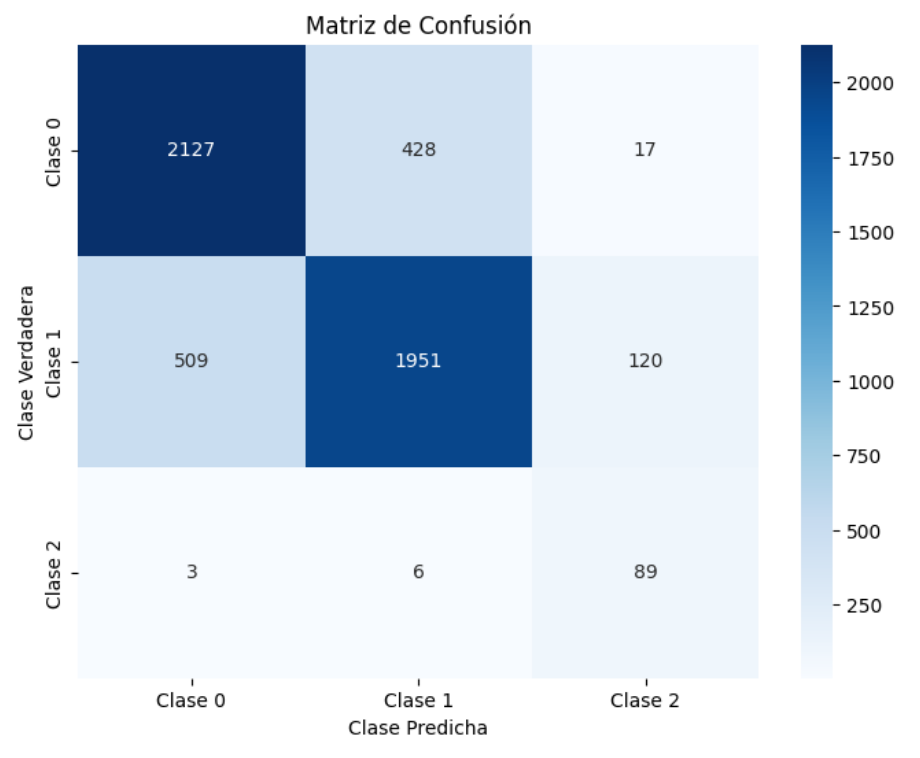
\includegraphics[width=0.8\textwidth]{capitulo5/figuras/matriz_confusion.PNG}
	\caption{Matriz de Confusión
		\\\textit{Fuente: Elaboracion Propia}}
	\label{fig:matriz}
\end{figure}

Los resultados de la matriz se pueden interpretar como:

\begin{itemize}

\item Clase 0:
Verdaderos Positivos (TP) = 2127
Falsos Negativos  (FN) = 428 + 17 = 445 (Ejemplos de clase 0 clasificados como 1 o 2)
Falsos Negativos Positivos (FP) = 509 + 3 = 512 (Ejemplos de clase 1 o 2 clasificados como 0)


\item Clase 1:
Verdaderos Positivos (TP) = 1951
Falsos Negativos (FN) = 509 + 120 = 629 (Ejemplos de clase 1 clasificados como 0 o 2)
Falsos Positivos (FP) = 428 + 6 = 434 (Ejemplos de clase 0 o 2 clasificados como 1)

\item Clase 2:
Verdaderos Positivos (TP) = 89
Falsos Negativos (FN) = 3 + 6 = 9 (Ejemplos de clase 2 clasificados como 0 o 1)
Falsos Positivos (FP) = 17 + 120 = 137 (Ejemplos de clase 0 o 1 clasificados como 2)

\end{itemize}

%\textbf{Análisis de las métricas de evaluación}

El análisis del desempeño del modelo cnn\_dp\_two revela los siguientes puntos importantes:

\begin{itemize}

\item Desempeño Desbalanceado:
El modelo muestra un buen desempeño en las Clases 0 y 1, con recall y precisión relativamente altos. 

\item Alta Precisión en Clase 2:
La Clase 2 muestra una alta precisión (aproximadamente 0.908), lo que indica que cuando el modelo predice la Clase 2, generalmente es correcto. Sin embargo, el bajo recall sugiere que no está detectando suficientes instancias de la Clase 2.

\item Falsos Positivos y Negativos:
Para la Clase 0 y la Clase 1, hay un número considerable de falsos positivos y falsos negativos. Esto sugiere que el modelo está confundiendo estas clases entre sí.


\end{itemize}


\section{DESPLIEGUE}
En esta sección se detalla la construcción de una aplicación de escritorio diseñada para la clasificación de comentarios textuales. Esta aplicación incluye la carga del mejor modelo previamente seleccionado, la matriz de embeddings y el tokenizador correspondiente. La misma permite al usuario ingresar un comentario que será procesado por el modelo clasificador, mostrando el resultado de la clasificación en la pantalla. Esta sección se compone de la siguiente carpeta:

La carpeta clasificadorcnn contiene los siguientes archivos:

\begin{itemize}

\item manipular\_modelo.py: Este archivo incluye funciones para cargar el tokenizador, la matriz de embeddings, ensamblar el modelo clasificador y preprocesar la entrada para realizar la predicción, para más detalles ver la figura \ref{fig:uml12}.

\begin{figure}[h!]
	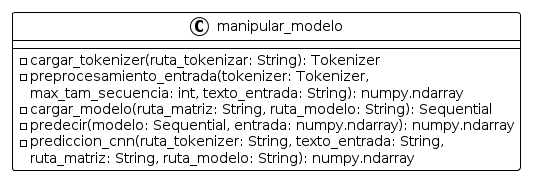
\includegraphics[width=0.8\textwidth]{capitulo5/figuras/fig12.png}
	\caption{Diagrama de clase del archivo manipular\_modelo.py
		\\\textit{Fuente: Elaboracion Propia}}
	\label{fig:uml12}
\end{figure}

\item interfaz.py: Este archivo se encarga de crear la interfaz de usuario, donde se ingresa el comentario a clasificar y se muestran los resultados de la clasificación, para más detalles ver la figura \ref{fig:uml13}.

\begin{figure}[h!]
	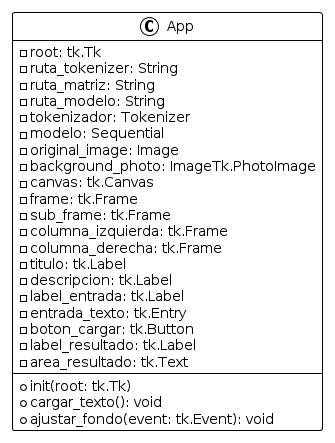
\includegraphics[width=0.5\textwidth]{capitulo5/figuras/fig13.png}
	\caption{Diagrama de clase del archivo interfaz.py
		\\\textit{Fuente: Elaboracion Propia}}
	\label{fig:uml13}
\end{figure}

\end{itemize}

Para simplificar la carga del modelo y hacer que los archivos sean más portables, se descompuso el modelo en varias partes:

\begin{itemize}

\item Matriz de embeddings: Se guardó en formato .npy, que es el formato nativo de la librería NumPy de Python, ampliamente utilizada en ciencia de datos y aprendizaje automático para cálculos numéricos. Este formato permite almacenar la matriz de manera eficiente y facilita su carga y uso posterior.

\item Pesos del modelo: Se almacenaron en formato .h5 (HDF5, Hierarchical Data Format version 5), un formato comúnmente usado para manejar datos de alta dimensión y ofrecer almacenamiento jerárquico. Esto permite reutilizar el modelo entrenado sin necesidad de volver a entrenarlo, ya que los pesos se pueden cargar directamente desde el archivo.

\item Tokenizador: Se guardó en formato .pickle, que es un formato binario utilizado en Python para la serialización y deserialización de objetos. Este formato es ideal para almacenar objetos complejos como los tokenizadores, que se usan en aplicaciones de procesamiento de lenguaje natural. La capacidad de .pickle para serializar prácticamente cualquier objeto Python, incluyendo listas, diccionarios y clases personalizadas, hace que sea una opción conveniente para este propósito.

\end{itemize}


\subsection{Implementación}
A continuación, se presenta el código fuente de cada archivo mencionado en la sección:

El código fuente \ref{lst:modelo} corresponde al archivo manipular\_modelo.py, donde se puede apreciar la implementación del cargado del modelo, su respectiva capa embedding con keras y el tokenizador con el módulo pickle de python para el preprocesado del texto de entrada.

\lstinputlisting[language=Python,firstline=7,caption=Codigo fuente del archivo manipular\_modelo.py
\\\textit{Fuente: Elaboracion Propia},label={lst:modelo}]{capitulo5/codigo/manipular_modelo.py}


El código fuente del archivo interfaz.py se desarrolló utilizando la librería Tkinter para crear una interfaz gráfica de usuario. Dado que es un componente secundario, no se proporcionarán detalles adicionales de este archivo.
\section{RECURSOS COMPUTACIONALES}
La implementación de los módulos diseñados y detallados anteriormente se llevó a cabo en dos computadoras personales y un servicio en la nube con las siguientes características:

Computadora Personal 1

\begin{itemize}

\item Procesador: Intel Core i7 no especificado
\item Memoria RAM: no especificada
\item Sistema Operativo: Windows 10
\item Tarjeta Gráfica: No especificada

\end{itemize}

Computadora Personal 2

\begin{itemize}

\item Procesador: MacBook Pro (modelo específico no indicado)
\item Memoria RAM: No especificada
\item Sistema Operativo: macOS Monterey
\item Tarjeta Gráfica: No especificada

\end{itemize}

Servicio en la Nube

\begin{itemize}

\item Recurso de Hardware: Acceso a GPUs y TPUs de alta calidad (T4, A100, L4 y TPU v2)
\item Memoria RAM: Amplia capacidad
\item Tiempo de Ejecución: Prolongado, mayor a 12 horas de ejecución
\item Sistema Operativo: Linux personalizado

\end{itemize}

En las siguientes subsecciones se detallan las herramientas de software utilizadas y la implementación llevada a cabo para la clasificación de comentarios, etiquetado de comentarios, creación, entrenamiento y uso de los modelos generados en el proceso de prueba.

\subsection{Herramientas de Software}
El lenguaje de programación utilizado es Python, elegido por su sintaxis clara y fácil de leer, lo que permite centrarse más en la lógica del código y menos en los detalles sintácticos. Además, Python cuenta con una amplia variedad de bibliotecas y frameworks específicos para el aprendizaje automático y análisis de datos, tales como TensorFlow, Keras, PyTorch, Scikit-learn, Matplotlib, Seaborn y Pandas. Todas estas herramientas ofrecen funciones avanzadas que facilitan el desarrollo de proyectos en esta área, asi como BERT. El mismo es el modelo utilizado para el etiquetado de texto, y significa Bidirectional Encoder Representations from Transformers. Es un modelo de lenguaje preentrenado desarrollado por Google, tiene una arquitectura compuesta por múltiples capas de transformers, que son unidades básicas que procesan secuencias de entrada de manera bidireccional. Esto significa que el modelo puede capturar el contexto de una palabra en una oración teniendo en cuenta tanto las palabras que la preceden como las que la siguen, lo que lo hace extremadamente efectivo para una amplia gama de tareas de procesamiento del lenguaje natural. Esto se logra mediante el entrenamiento del modelo en dos tareas: 

\begin{itemize}
\item El modelado de lenguaje enmascarado (Masked Language Modeling, MLM) que ocurre durante el entrenamiento, donde BERT recibe una secuencia de palabras de entrada y algunas de estas palabras son enmascaradas aleatoriamente. La tarea del modelo es predecir qué palabra falta en cada lugar enmascarado, lo que obliga al modelo a comprender el contexto de las palabras en una oración para poder predecir la palabra enmascarada con precisión. Ver figura \ref{fig:nlp8}

\item Predicción de la siguiente oración: Además del MLM, BERT también se entrena en una tarea de predicción de la siguiente oración. Se le proporcionan dos oraciones y el modelo debe predecir si la segunda oración sigue a la primera en un contexto coherente o no.
\end{itemize}

\begin{figure}[h!]
	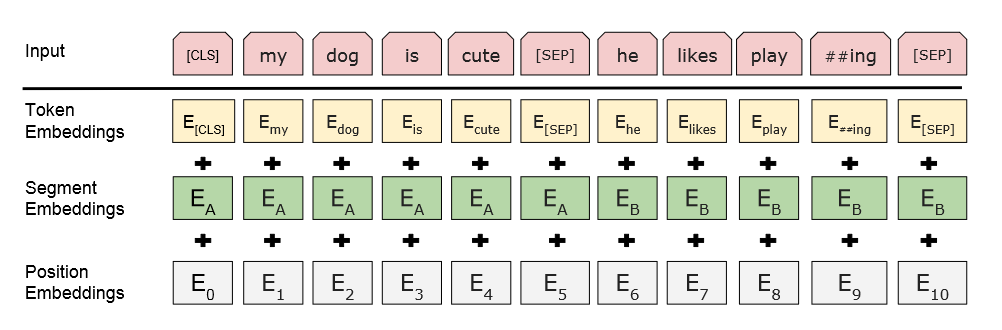
\includegraphics[width=0.65\textwidth]{capitulo3/figuras/nlp8.png}
	\caption[Representacion de entradas en BERT.]{Representacion de entradas en BERT.
		\\\textit{Fuente: Extraído de} \protect\cite[p. 5]{devlin2018bert} }
	\label{fig:nlp8}
\end{figure}

Para este proyecto, se utilizó la versión específica de BERT denominada ``bert\_uncased\_L-4\_H-512\_A-8'', una de las 24 variantes del conjunto ``BERT miniatura''. Estos modelos son versiones más compactas del BERT original, con una arquitectura reducida en comparación con BERT base o BERT grande, como se muestra en la tabla \ref{tbl:1}. Esto significa que tienen menos parámetros y requieren menos recursos computacionales para su entrenamiento y ejecución. Dado que los recursos necesarios para trabajar con un BERT base no están disponibles para este proyecto, utilizar este modelo compacto resultó extremadamente útil.

El modelo ``bert\_uncased\_L-4\_H-512\_A-8'' se entrena con texto en minúsculas, de ahí su denominación ``uncased''. Cuenta con cuatro capas (indicadas por ``L-4''), una dimensión de representación oculta de 512 en cada capa (indicada por ``H-512'') y utiliza ocho cabezas de atención en la capa de atención multi-cabeza (representadas por ``A-8'').

\begin{table}[!ht]
	\centering
	\caption[Representacion de versiones de BERT]{Representacion de versiones de BERT
		\\\textit{Fuente: Elaboracion Propia}}
	\begin{tabular}{|c|>{\centering\arraybackslash}m{2.5cm}|>{\centering\arraybackslash}m{2.5cm}|>{\centering\arraybackslash}m{3cm}|>{\centering\arraybackslash}m{2.5cm}|}
		\hline
		\textbf{} & \textbf{H=128} & \textbf{H=256} & \textbf{H=512} & \textbf{H=768} \\ \hline
		\textbf{L=2} & \makecell{2/128 \\ (BERT-Tiny)} & 2/256 & 2/512 & 2/768 \\ \hline
		\textbf{L=4} & 4/128 & \makecell{4/256 \\ (BERT-Mini)} & \makecell{4/512 \\ (BERT-Small)} & 4/768 \\ \hline
		\textbf{L=6} & 6/128 & 6/256 & 6/512 & 6/768 \\ \hline
		\textbf{L=8} & 8/128 & 8/256 & \makecell{8/512\\(BERT-Medium)} & 8/768 \\ \hline
		\textbf{L=10} & 10/128 & 10/256 & 10/512 & 10/768 \\ \hline
		\textbf{L=12} & 12/128 & 12/256 & 12/512 & \makecell{12/768 \\ (BERT-Base)} \\ \hline
	\end{tabular}
	\label{tbl:1}
\end{table}


Para cada tarea que se desee realizar con BERT, es crucial seleccionar los mejores hiperparámetros de ajuste a partir de las siguiente tabla \ref{tbl:2}:

\begin{table}[!ht]
	\centering
	\begin{tabular}{|c|c|}
		\hline
		\textbf{Hiperparametros} & \textbf{Valores} \\ \hline
		Tamaños de lote & 8, 16, 32, 64, 128 \\ \hline
		Tasas de aprendizaje & 3e-4, 1e-4, 5e-5, 3e-5 \\ \hline
		Número de épocas &  1, 2, 3, 4, 5 \\ \hline
		Tipo de capa de preprocesamiento & Según el modelo a usar \\ \hline
	\end{tabular}
	\caption[Detalle de hiperparametros y sus valores en BERT]{Detalle de hiperparametros y sus valores en BERT
		\\\textit{Fuente: Elaboracion Propia}}
	\label{tbl:2}
\end{table}

En este proyecto, para la tarea de etiquetado de los conjuntos de datos, se optó por un modelo de preprocesamiento ya entrenado específicamente seleccionado. La configuración específica incluyó:

\begin{itemize}

\item Capa de preprocesamiento: Una capa codificadora entrenable que se actualiza durante el entrenamiento(en-uncased-preprocess-version-3).
\item Capa de abandono: Con una tasa de abandono del 10\%.
\item Capa densa: Con una función de activación softmax para la clasificación múltiple.
\item Tamaño de lote: 32, lo que significa que los datos se dividen en lotes más pequeños con ese tamaño.
\item Tasa de aprendizaje: 3e-5.
\item Optimizador: AdamW.
\item Número de épocas: 5.

\end{itemize}

Para evaluar el modelo, se obtuvieron la pérdida y la precisión del modelo en el conjunto de prueba.

El entrenamiento del modelo BERT, el proceso de etiquetado de datos y la creación y entrenamiento de modelos de redes convolucionales se llevaron a cabo utilizando Google Colab (abreviatura de Colaboratory), una plataforma en línea proporcionada por Google. Colab permite escribir y ejecutar código Python en un entorno de cuaderno basado en la nube de forma gratuita como se muestra en la figura \ref{fig:bertito}. Está diseñado para facilitar la colaboración en proyectos de ciencia de datos y aprendizaje automático, así como para el desarrollo y experimentación con código Python sin necesidad de configurar un entorno local.

Google Colab ofrece acceso gratuito a recursos de cómputo en la nube, incluidas unidades de procesamiento gráfico (GPU) y unidades de procesamiento tensorial (TPU). Estos recursos fueron utilizados para el etiquetado de los conjuntos de datos. Sin embargo, el uso gratuito de CPU, GPU y TPU tiene limitaciones. Estas limitaciones se hicieron evidentes al entrenar el modelo BERT con grandes cantidades de datos, ya que el proceso requería mucho más tiempo de entrenamiento y el entorno se desconectaba, dejando el entrenamiento incompleto. Para evitar este problema, se adquirió el paquete Colab Pro, el cual garantiza que el entorno de ejecución no se desconecte y permite que BERT complete su entrenamiento sin interrupciones.

\begin{figure}[h!]
	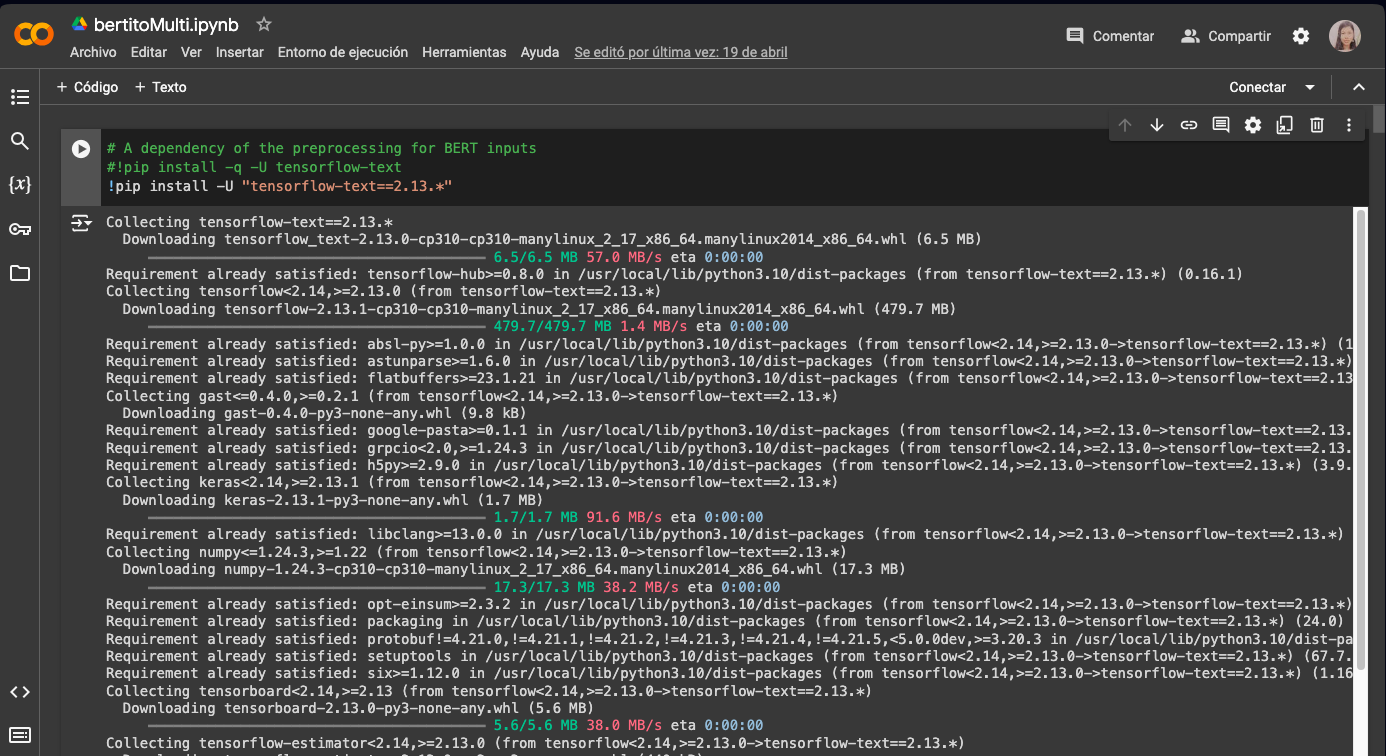
\includegraphics[width=1\textwidth]{capitulo5/figuras/bertito.png}
	\caption[Formato de cuaderno colab instalando libreria tensorflow-text-2.13]{Formato de cuaderno colab instalando libreria tensorflow-text-2.13
		\\\textit{Fuente: Elaboracion Propia}}
	\label{fig:bertito}
\end{figure}

Para la creación de los modelos de redes neuronales convolucionales se utilizó Keras, una API de alto nivel recomendada para TensorFlow a partir de su versión 1.14. Keras es una biblioteca de código abierto para la creación y entrenamiento de modelos de redes neuronales en Python. Es conocida por su facilidad de uso, ya que proporciona una interfaz de alto nivel que simplifica la construcción y el entrenamiento de modelos de redes neuronales. Los modelos de Keras se construyen utilizando capas que se pueden apilar o combinar de diversas formas para crear arquitecturas complejas.

A continuación, se detallan las versiones y bibliotecas utilizadas:

\begin{itemize}

\item Keras: 2.15.0
\item Matplotlib: 3.1.1
\item NumPy: 1.17.4
\item Python: 3.11.4
\item TensorFlow: 2.13.0 (para el modelo BERT)
\item Tensor-text: 2.13.0 (para el modelo BERT)
\item TensorFlow: 2.15.0 (para otros modelos)

\end{itemize}




